\documentclass[12pt]{article}
\textheight 22.00cm           
\textwidth 17.00cm            
\oddsidemargin 0cm
\topmargin 0cm
\usepackage{rotating}
\usepackage[official]{eurosym}
\usepackage{enumitem}
\usepackage{tabularx}
\usepackage{array}
\usepackage{multicol}

\pagestyle{headings}
\markright{Ryan Cloutier}

\begin{document}
\thispagestyle{empty}
\centerline{{\large\bf Curriculum Vitae}}
\vspace{2ex}

\centerline{\bf Ryan Edward Cloutier}
\subsubsection*{Business Address}

Department of Physics \& Astronomy \\
McMaster University \\
1280 Main Street W. \\
Hamilton, ON \\
L8S 4L8 \\
\\
ABB -- 317A \\
(905) 525-9140 x27860 \\ 
ryan.cloutier@mcmaster.ca

\subsubsection*{Educational Background}
Hon. B.Sc., Physics \& Astronomy, University of Toronto, 2014\\
Ph.D., Astronomy \& Astrophysics, University of Toronto, 2019 
% (supervisors R. Doyon \& K. Menou)

\subsubsection*{Current Status at McMaster}
Assistant Professor, Department of Physics \& Astronomy \\
Canada Research Chair in Exoplanetary Astronomy (Tier 2) 


\subsubsection*{Employment History}

\begin{tabbing}
\hspace{2.5cm} 	\= \kill
2022-: \> Assistant Professor, Department of Physics \& Astronomy, McMaster University \\
\> Hamilton, ON \\
2021-22: \> Banting Fellow, Center for Astrophysics $|$ Harvard \& Smithsonian, \\
\> Cambridge, MA, USA \\
2019-21: \> Postdoctoral Fellow, Center for Astrophysics $|$ Harvard \& Smithsonian, \\
\> Cambridge, MA, USA \\
\end{tabbing}

\subsubsection*{Honours \& Awards}
\begin{itemize}[noitemsep]
\item Canada Research Chair in Exoplanetary Astronomy (Tier 2), 2025-30
\begin{itemize}
\item Federal appointments for exceptional emerging researchers, acknowledged by their peers as having the potential to lead in their field.
\end{itemize}
\item John C. Polanyi Prize in Physics, 2023
\begin{itemize}
\item Awarded by the Government of Ontario to outstanding reseachers in the early stages of their careers in the categories of the Noble Prize.  
\end{itemize}
\item Allen Yen Award, 2018
\begin{itemize}
\item Awarded to a graduate student in the University of Toronto's Department of Astronomy \& Astrophysics who has undertaken ``particularly notable research".
\end{itemize}
\item Lachlan Gilchrist Fellowship, 2015-19
\begin{itemize}
\item Awarded to a graduate student in a Physical Sciences program at the University of Toronto on the basis of academic merit.
\end{itemize}
\item Mary H. Beatty Scholarship, 2014-15 
\begin{itemize}
\item Entrance scholarship for graduate students at the University of Toronto.
\end{itemize}
\end{itemize}

\subsubsection*{Research Impact}
\begin{itemize}[noitemsep]
\item Number of co-authored, peer-reviewed articles (published + in press): 117
\item Number of citations: 4,130
\item h-index: 41
%\item Top five cited papers with major involvement by {\bf Ryan Cloutier} (number of citations):
%\begin{itemize}[noitemsep]
%\item {\bf Cloutier, R.}, \& Menou, K. 2020. ``Evolution of the Radius Valley around Low-mass Stars from Kepler and K2''. {\it The Astronomical Journal}, 159, 211 (183)
%\item Currie, T., {\bf Cloutier, R.}, Brittain, S., Grady, C., Burrows, A., et al. 2015. ``Resolving the HD 100546 Protoplanetary System with the Gemini Planet Imager: Evidence for Multiple Forming, Accreting Planets". {\it The Astrophysical Journal}, 814, 27 (142)
%\item {\bf Cloutier, R.}, Astudillo-Defru, N., Doyon, R., Bonfils, X., Almenara, J. -M., Benneke, B., et al. 2017. ``Characterization of the K2-18 multi-planetary system with HARPS: A habitable zone super-Earth and discovery of a second, warm super-Earth on a non-coplanar orbit''. {\it Astronomy \& Astrophysics}, 608, 35 (98)
%\item {\bf Cloutier, R.}, Eastman, J. D., Rodriguez, J. E., Astudillo-Defru, N., Bonfils, X., Mortier, A., et al. 2020. ``A Pair of TESS Planets Spanning the Radius Valley around the Nearby Mid-M Dwarf LTT 3780''. {\it The Astronomical Journal}, 160, 3 (94)
%\item {\bf Cloutier, R.}, Astudillo-Defru, N., Doyon, R., Bonfils, X., Almenara, J. -M., Bouchy, F., et al. 2019. ``Confirmation of the radial velocity super-Earth K2-18c with HARPS and CARMENES''. {\it Astronomy \& Astrophysics}, 621, 49 (78)
%\item Nelson, B. E., Ford, E. B., Buchner, J., {\bf Cloutier, R.}, Díaz, R. F., Faria, J. P., et al. (2020). ``Quantifying the Bayesian Evidence for a Planet in Radial Velocity Data''. {\it The Astronomical Journal}, 159, 73 (82)
%\item {\bf Cloutier, R.}, Astudillo-Defru, N., Bonfils, X., Jenkins, J. S., Berdiñas, Z., Ricker, G., et al. 2019. ``Characterization of the L 98-59 multi-planetary system with HARPS: Mass characterization of a hot super-Earth, a sub-Neptune, and a mass upper limit on the third planet''. {\it Astronomy \& Astrophysics}, 629, 111 (72)
%\end{itemize}
\end{itemize}

\begin{figure}[h!]
\centering
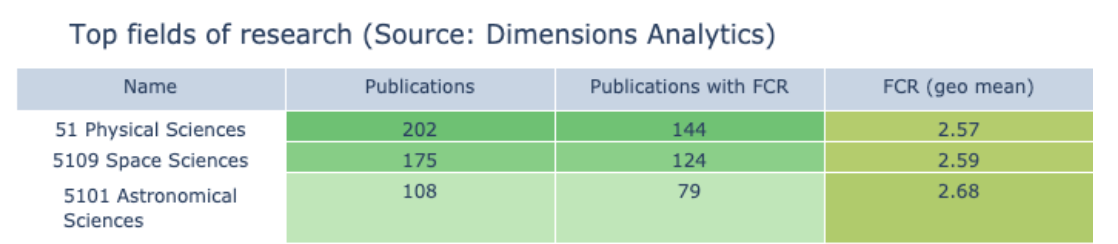
\includegraphics[width=0.9\hsize]{fcr.png}
\caption{Field Citation Ratio (FCR) expresses the citation-based impact of the publication set relative to publications from the same research area and year. FCR=1 implies that publications are cited as often as expected based on publication year and research area. FCR=2 implies that publications are cited twice as often as expected based on publication year and research area. \textbf{Note:} References to datasets are counted here as ``Publications with FCR", which are rarely cited in publications. The FCR values from peer-reviewed publications only are therefore higher than the FCR values reported here. (\emph{Date: July 29, 2026})}
\end{figure}

\begin{figure}[h!]
\centering
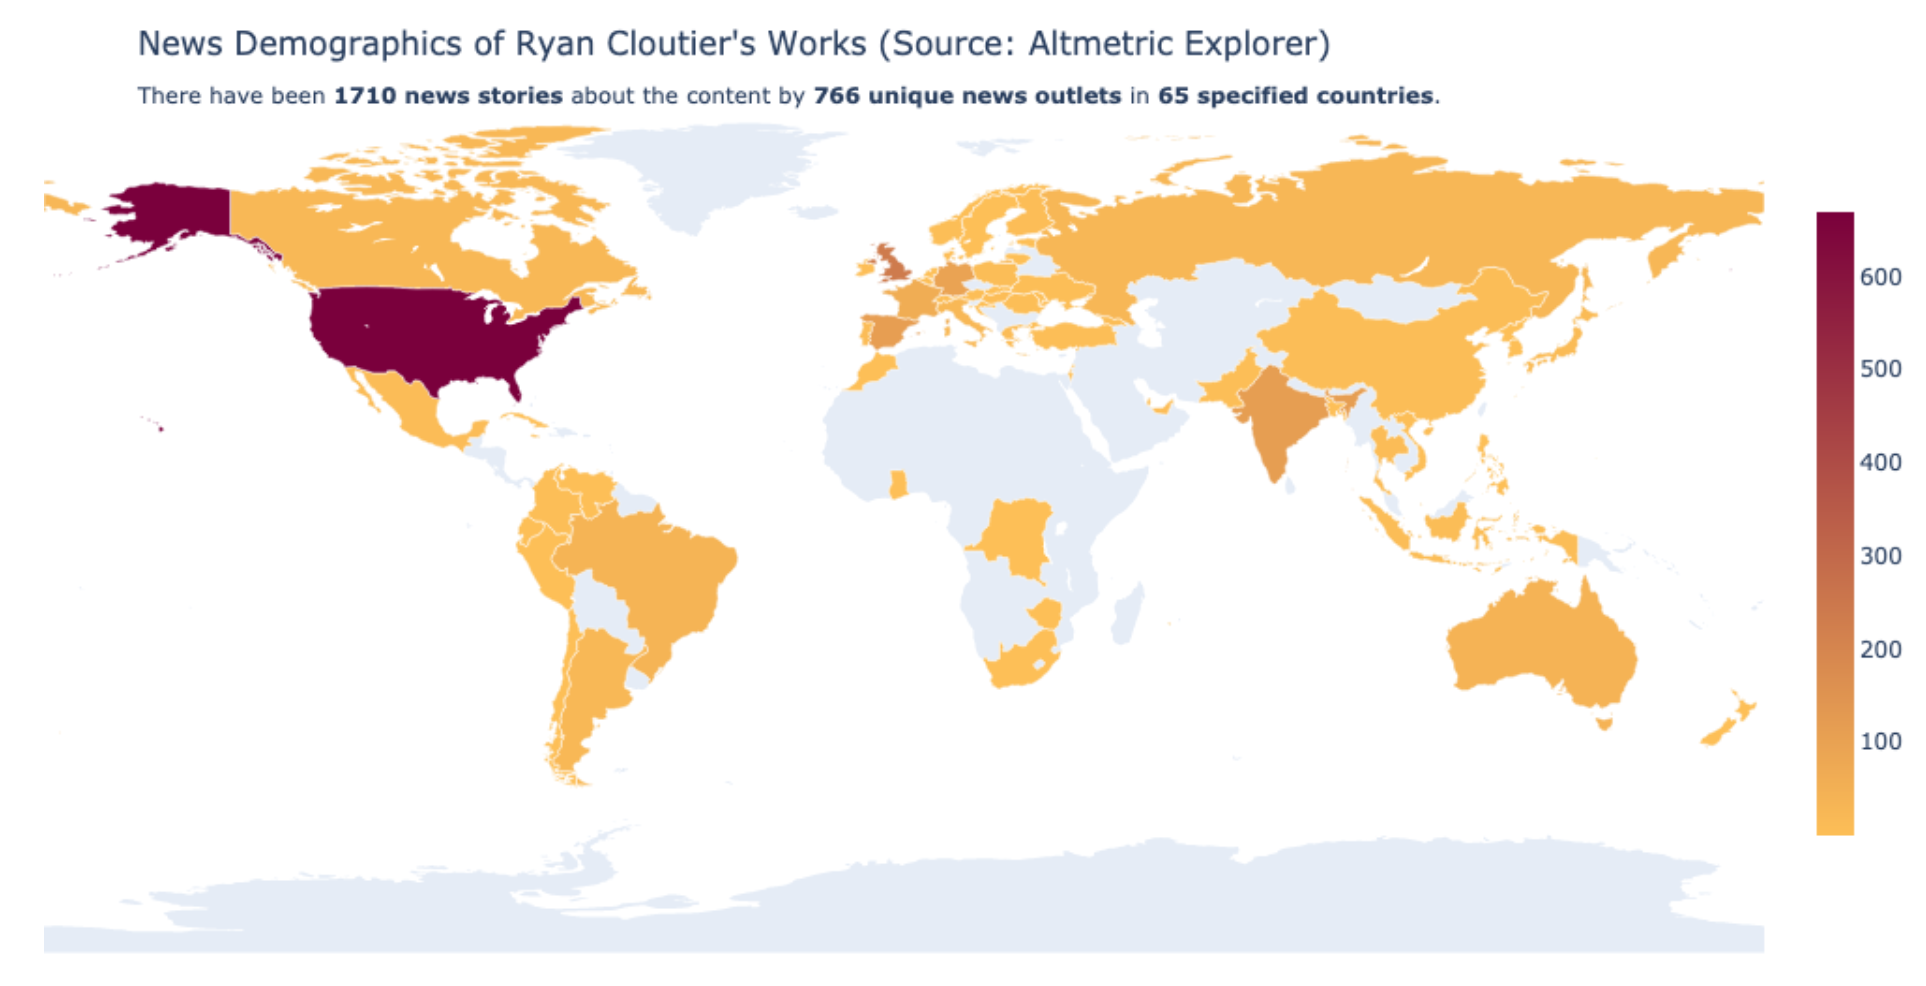
\includegraphics[width=0.49\hsize]{news.png}
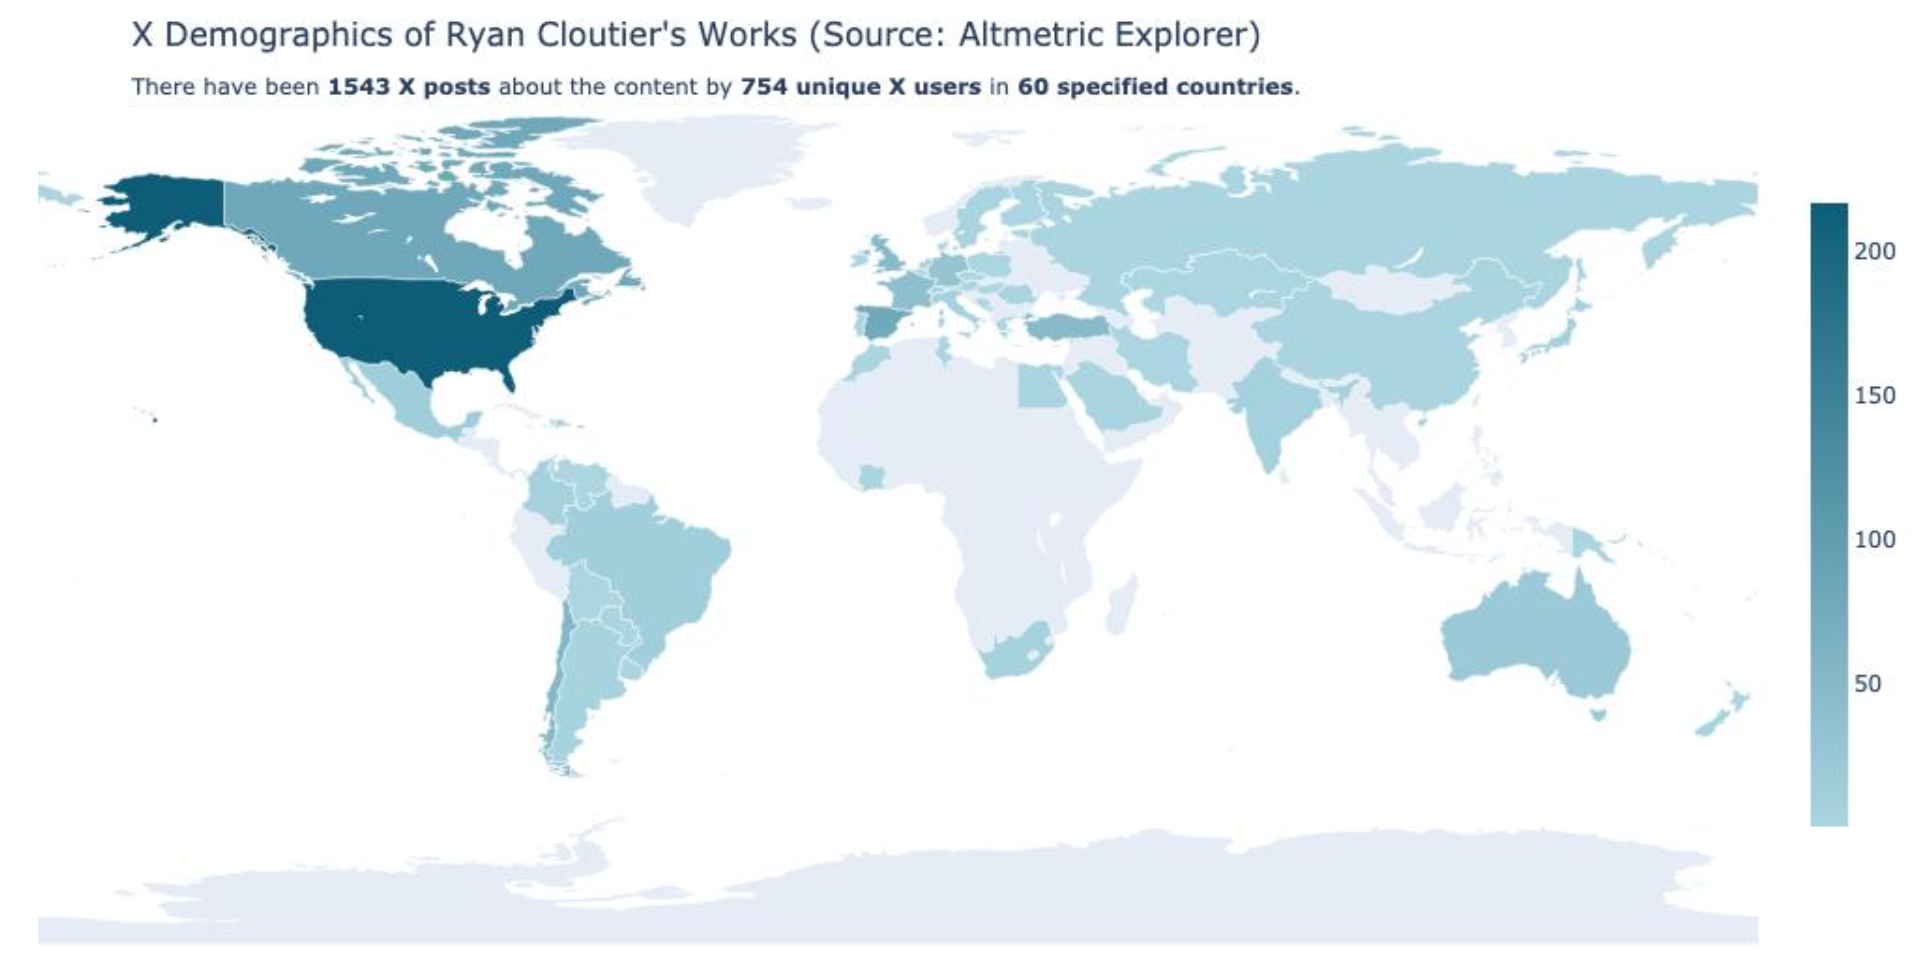
\includegraphics[width=0.49\hsize]{socialmedia.png}
\caption{Broader research impacts as depicted by mentions in online news stories (\emph{top}) and X social media posts (\emph{bottom}) across the globe. (\emph{Date: July 29, 2026})}
\end{figure}



%\noindent {\bf Editor of Conference Proceedings}
%\begin{itemize}
%\item Co-Editor, ``Star Clusters: from the Milky Way to the Early Universe'' International Astronomical Union symposium, Bologna, May 2019
%\end{itemize}

\newpage
\subsubsection*{Areas of Interest \& Research Topic Network}

\begin{multicols}{2} % Starts a 2-column layout
    \begin{itemize}[noitemsep]
        \item Exoplanetary Astronomy
        \item Exoplanet Detection Methods
        \item Exoplanet Demographics
        \item Planet Formation
        \item Planetary Interiors
        \item Planetary Atmospheres
        \item Observational Astronomy
        \item Stellar Astrophysics
        \item Low Mass Stars
        \item Stellar Chemical Abundances
        \item Stellar Magnetic Activity
        \item Stellar Winds
    \end{itemize}
\end{multicols}


\begin{figure}[h!]
\centering
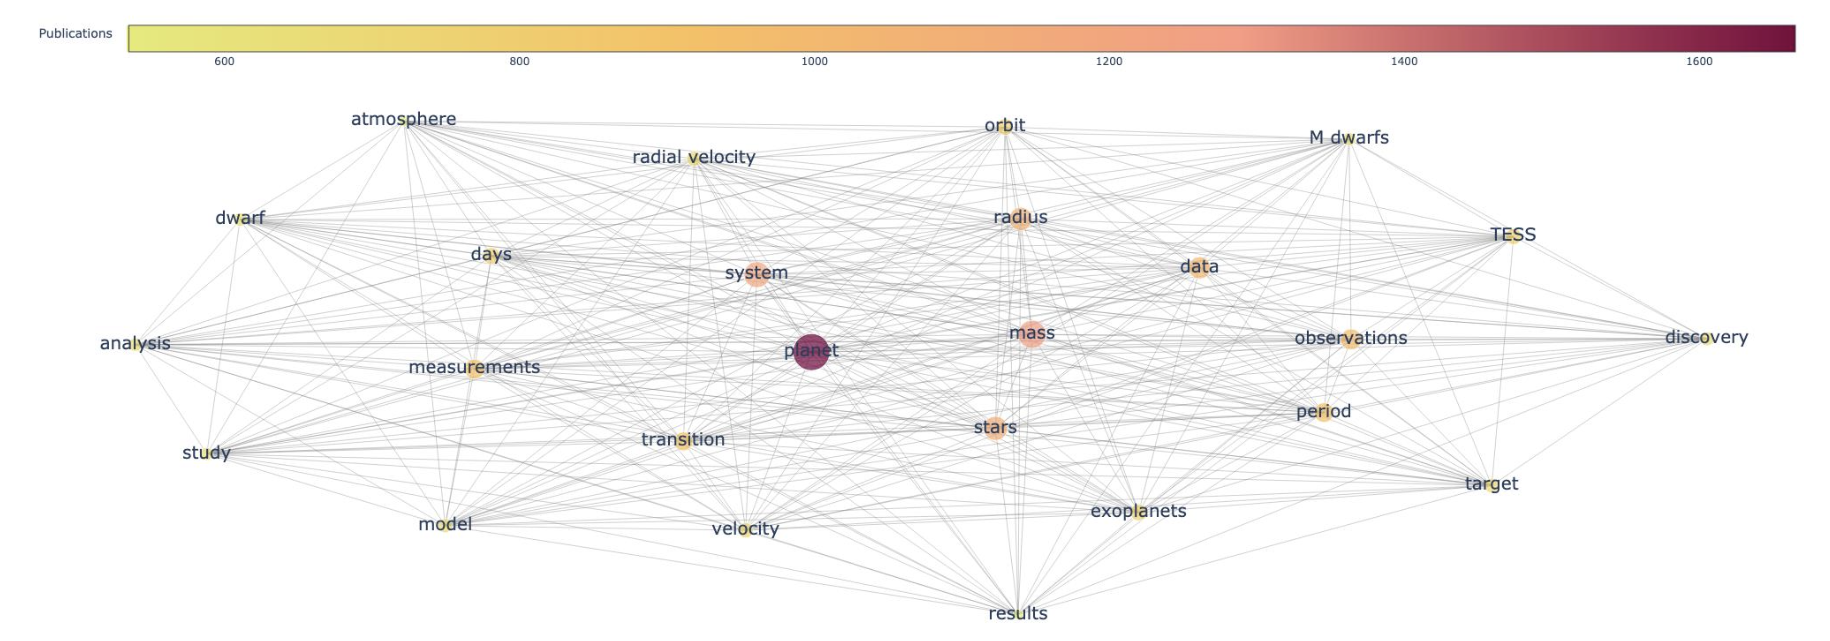
\includegraphics[width=\hsize]{research_network.png}
\caption{Research topic network drawn from mentions in peer-reviewed publications. (\emph{Date: July 29, 2026})}
\end{figure}

\newpage
\subsubsection*{Lifetime Publications}

\begin{figure}[h!]
\centering
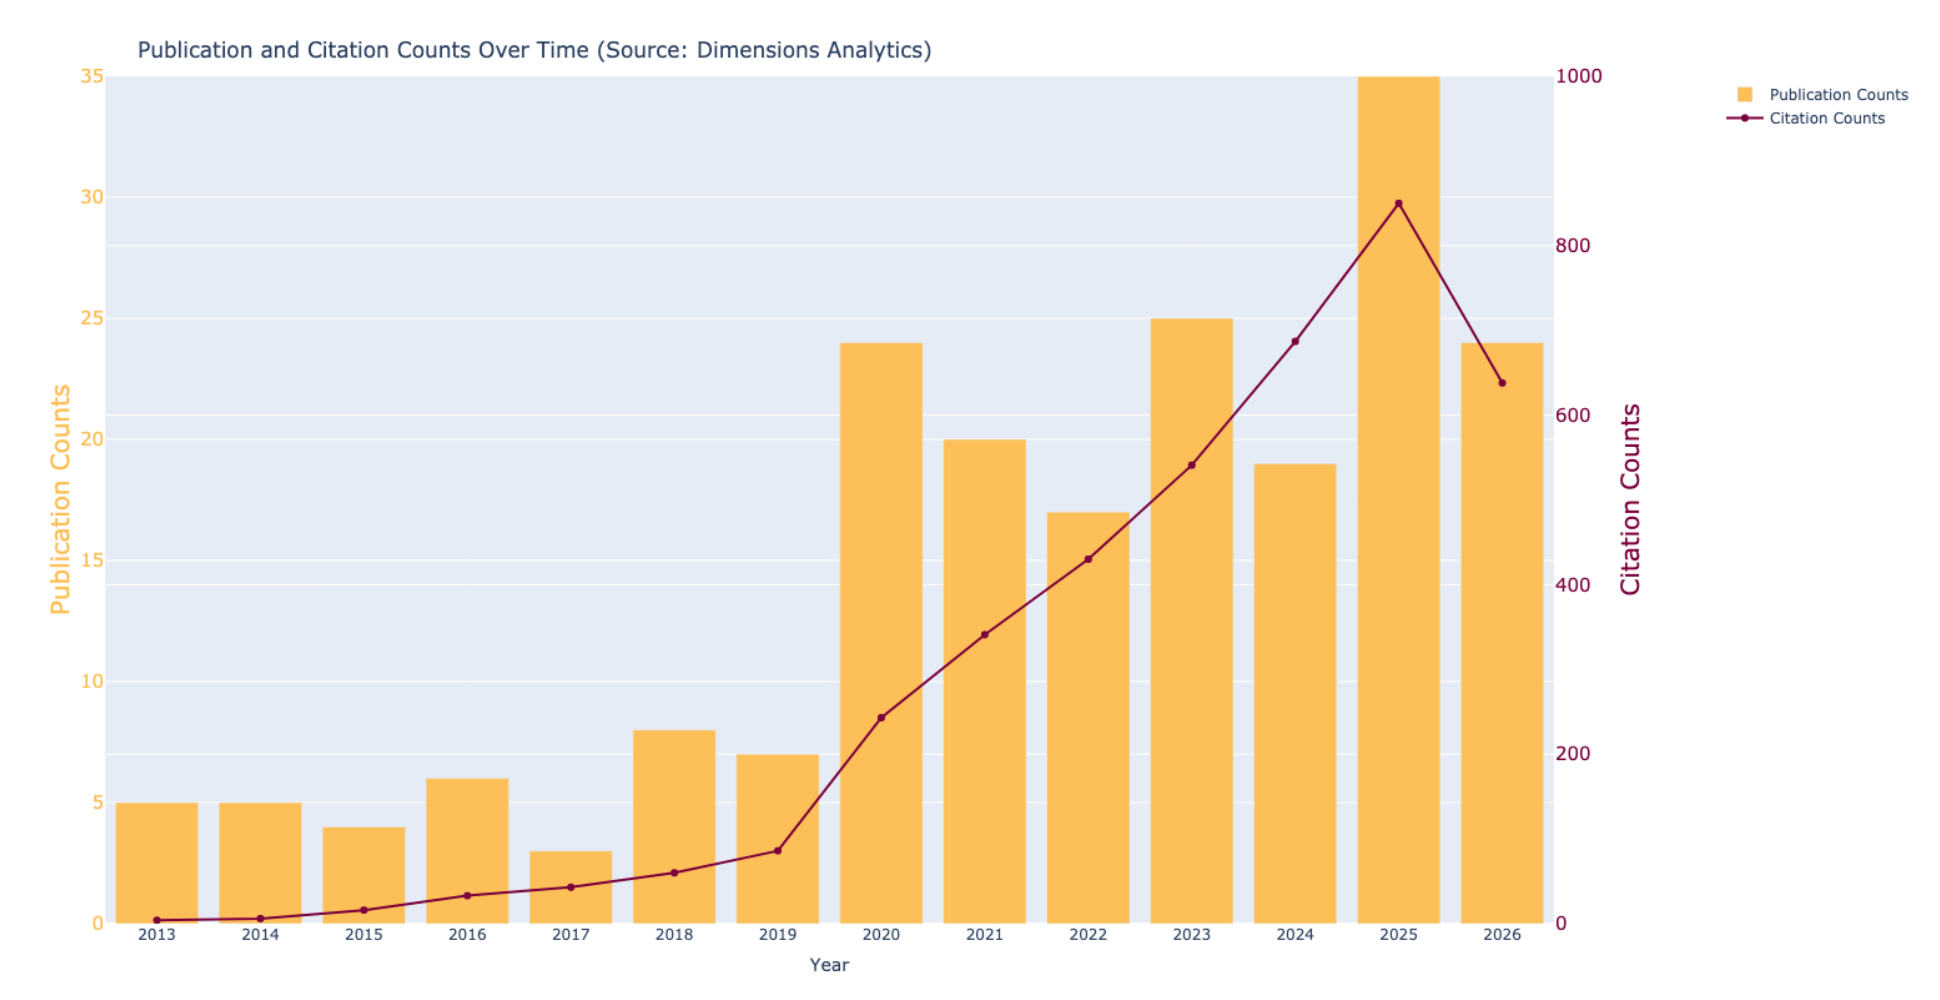
\includegraphics[width=0.8\hsize]{citations.png}
\caption{Per annum publications and citations since \textbf{R. Cloutier} entered the field in 2013. (\emph{Date: July 29, 2026})}
\end{figure}

\noindent Students and postdoctoral fellows that I have directly supervised are \underline{underlined}. The first author of each paper is the corresponding author.


\begin{itemize}
\item Book Chapters
\begin{enumerate}
\item {\bf Cloutier, R.} ``Exoplanet Demographics: Physical \& Orbital Properties'', Chapter 1 of {\it Encyclopedia of Astrophysics, Volume 1}, Elsevier Publishing, 2026.
\end{enumerate}

\item Peer-Reviewed Journal Articles

\begin{enumerate}
\item \underline{Skinner, B.N.}, Pudritz, R.E., \& {\bf Cloutier, R.} (2026) ``A validated low-to-intermediate mass planetary interior structure model and new mass-radius relations,'' {\it  Monthly Notices of the Royal Astronomical Society}, 550, 3.
\item \underline{Turtelboom, E.V.}, Giacalone, S., Gore, R., Dressing, C.D., {\bf Cloutier, R.}, et al., ``Uniform Metallicity Measurements of M Dwarf Planet Hosts Support Metallicity-Dependent Sub-Neptune Formation'' {\it The Astronomical Journal}, 172, 121.
\item Thompson, W., Blakely, D., Xuan, J.W., Blouin, S., Zhang, J., et al. (2026), ``Detecting and Characterizing Companions with a Calibrated Gaia DR2, DR3, and Hipparcos Catalog (G23H),'' {\it The Astronomical Journal}, 172, 53.
\item Pelletier, S., Allart, R., Vaulato, V., Ehrenreich, D., Cristo, E., et al. (2026), ``The breaking of cold traps and onset of titanium in ultra-hot Jupiter atmospheres: WASP-189b in context,'' {\it Astronomy \& Astrophysics}, 711, 119.
\item \underline{Gillis, E.D.}, {\bf Cloutier, R.}, \& Pass, E.K. (2026), ``TESS Planet Occurrence Rates Reveal the Disappearance of the Radius Valley around Mid-to-late M Dwarfs,'' {\it The Astronomical Journal}, 171, 317.
\item \underline{Weisserman, D.}, \underline{Gromek, N.}, {\bf Cloutier, R.}, Bali, K., Cadieux, C., et al. (2026), ``Super-Earth masses and stellar abundances from NIRPS reveal tentative evidence for water-rich formation around M dwarfs,'' {\it Astronomy \& Astrophysics}, 709, 165.
\item Srivastava, A., Doyon, R., Bouchy, F., Artigau, E., Cadieux, C., et al. (2026), ``TOI-4552 b: A new ultra-short-period rocky world revealed by NIRPS and TESS,'' {\it Astronomy \& Astrophysics}, 709, 73.
\item \underline{Osborn, A.}, {\bf Cloutier, R.}, Bourrier, V., \underline{Skinner, B.}, \underline{Gromek, N.}, et al. (2026), ``Confirmation of the hot super-Neptune TOI-672 b with NIRPS and HARPS: Insights into the Neptunian desert around M dwarfs,'' {\it Astronomy \& Astrophysics}, 709, 23
\item Parc, L., Cadieux, C., Grieves, N., Bouchy, F., L'Heureux, A., et al. (2026), ``Densities of small planets around the M dwarfs TOI-4336 A and TOI-4342 with ESPRESSO: Three sub-Neptunes, one super-Earth, and a Neptune-mass candidate,'' {\it Astronomy \& Astrophysics}, 708, 81
\item Frensch, Y., Bouchy, F., Lo Curto, G., L'Heureux, A., de Lima Gomes, R., et al. (2026), ``TOI-3288 b and TOI-4666 b: two gas giants transiting low-mass stars characterised by NIRPS", {\it Astronomy \& Astrophysics}, 707, 73.
\item \underline{Rochon, A.}, Artigau, E., \underline{Weisserman, D.}, Dang, L., Doyon, R., et al. (2026), ``Reanalysis of the Eclipses of LHS 1140 c: No Evidence of an Atmosphere and Implications for the Internal Structure of the Planet,'' {\it The Astrophysical Journal Letters}, 998, L39.
\item Lamontagne, P., \underline{Weisserman, D.}, Cadieux, C., Lafreni\`ere, D., L'Heureux, A., et al. (2026) ``NIRPS tightens the mass estimate of GJ 3090 b and detects a planet near the stellar rotation period'', {\it Astronomy \& Astrophysics}, 706, 278.
\item Wilson, T.G., \underline{Simpson, A.M.}, Collier Cameron, A., {\bf Cloutier, R.}, Adibekyan, V., et al. (2026), ``Gas-depleted planet formation occurred in the four-planet system around the red dwarf LHS 1903,'' {\it Science}, 392, 6795.
\item Turner, D., Eschen, Y., Murgas, F., Mortier, A., Wilson, T., et al. (2026) ``The mass of the exo-Venus Gliese 12 b, as revealed by HARPS-N, ESPRESSO, and CARMENES", {\it Monthly Notices of the Royal Astronomical Society}, 1703, 1608.
\item Ould-Elhkim, M., Moutou, C., Donati, J., Delfosse, X., Artigau, E., et al. (2026), ``The SPIRou Legacy Survey: Detection of a nearby world orbiting in the habitable zone of Gl 725B achieved by correcting strong telluric contamination in near-infrared radial velocities with wapiti,'' {\it Astronomy \& Astrophysics}, 705, 234.
\item \underline{Weisserman, D.}, \underline{Gillis, E.}, \textbf{Cloutier, R.}, Brown, N., Bean, J., et al. (2025) ``Aligned Stellar Obliquities for Two Hot Jupiter-hosting M Dwarfs Revealed by MAROON-X: Implications for Hot Jupiter Formation", {\it The Astronomical Journal}, 170, 313.
\item C\^ot\'e, P., Woods, T., Hutchings, J., Rhodes, J., S\`anchez-Janssen, R., et al. (2025) ``The CASTOR Mission", JATIS, in press.
\item Vaulato, V., Hobson, M., Allart, R., Pelletier, S., Wardenier, J., Chakraborty, H., et al. (2025) ``Atmospheric composition and circulation of the ultra-hot Jupiter WASP-121b with joint NIRPS, HARPS and CRIRES+ transit spectroscopy", {\it Astronomy \& Astrophysics}, 703, 251.
\item Coulombe, L.P., Benneke, B., Krissansen-Totton, J., L'Heureux, A., Piaulet-Ghorayeb, C., et al. (2025) ``Possible Evidence for the Presence of Volatiles on the Warm Super-Earth TOI-270 b", {\it The Astronomical Journal}, 170, 226.
\item Parc, L., Bouchy, F., Cook, N., Grieves, N., Artigau, \'E., et al. (2025) ``NIRPS and TESS reveal a peculiar system around the M dwarf TOI-756: A transiting sub-Neptune and a cold eccentric giant", {\it Astronomy \& Astrophysics}, 702, 138.
\item Yee, S., Winn, J., Hartman, J., Rodriguez, J., Zhou, G., et al. (2025) ``The TESS Grand Unified Hot Jupiter Survey. III. Thirty More Giant Planets", {\it The Astrophysical Journal Supplement Series}, 280, 30.
\item Cadieux, C., L'Heureux, A., Piaulet-Ghorayeb, P., Doyon, R., Artigau, \'E., et al. (2025) ``Detailed Architecture of the L 98-59 System and Confirmation of a Fifth Planet in the Habitable Zone", {\it The Astronomical Journal}, 170, 154.
\item Bazinet, L., Allart, R., Benneke, B., Pelletier, S., Wardenier, J., et al. (2025) ``Quantifying thermal water dissociation in the dayside photosphere of WASP-121 b using NIRPS", {\it Astronomy \& Astrophysics}, 701, 276.
\item Hesse, K., Mireles, I., Bouchy, F., Dragomir, D., Ulmer-Moll, S., et al. (2025) ``HD 35843: A Sun-like Star Hosting a Long-period Sub-Neptune and Inner Super-Earth", {\it The Astronomical Journal}, 170, 108.
\item Carmona, A., Delfosse, X., Ould-Elhkim, M., Cortes-Zuleta, P., Hara, N., et al. (2025) ``Characterizing planetary systems with SPIRou: Detection of mini-Neptune in a 6 day period orbit around the M dwarf Gl 410'', {\it Astronomy \& Astronphysics}, 700, 222.
\item Gomes da Silva, J., Delgado-Mena, E., Santos, N., Monteiro, T., Laure, P., et al. (2025) ``Blind search for activity-sensitive lines in the near-infrared using HARPS and NIRPS observations of Proxima and Gl 581'', {\it Astronomy \& Astronphysics}, 700, 177.
\item Suarez-Mascereno, A., Artigau, \'E, Mignon, L., Delfosse, X., Cook, N., et al. (2025) ``Diving into the planetary system of Proxima with NIRPS: Breaking the meter per second barrier in the infrared", {\it Astronomy \& Astrophysics}, 700, 11.
\item Bouchy, F., Doyon, R., Pepe, F., Melo, C., Artigau, \'E., et al. (2025) ``NIRPS joining HARPS at ESO 3.6 m: On-sky performance and science objectives", {\it Astronomy \& Astrophysics}, 700, 10.
\item Vaulato, V., Pelletier, S., Ehrenreich, D., Allart, R., Cristo, E., et al. (2025) ``Hydride ion continuum hides absorption signatures in the NIRPS near-infrared transmission spectrum of the ultra-hot gas giant WASP-189b", {\it Astronomy \& Astrophysics}, 700, 9.
\item Allart, R., Carteret, Y., Bourrier, V.,Mignon, L., Baron, F., et al. (2025) ``NIRPS detection of delayed atmospheric escape from the warm and misaligned Saturn-mass exoplanet WASP-69 b", {\it Astronomy \& Astrophysics}, 700, 7.
\item Ahrer, E., Radica, M., Piaulet-Ghorayeb, C., Raul, E., Wiser, L., et al. (2025) ``Escaping Helium, Depleted Methane, and Hints of Carbon Dioxide Suggest a High-Metallicity Atmosphere on Sub-Neptune GJ 3090 b from JWST Transit Spectroscopy'', {\it The Astronomical Journal}, 985, 10.
\item Wilson, T.G., \underline{Simpson, A.}, Collier-Cameron, A., {\bf Cloutier, R.}, Adibekyan, V., et al. (2025) ``The thick disk M-dwarf LHS 1903 contains a non-gaseous planet above the radius valley and three interior bodies'', {\it Science}, in press.
\item Ould-Elhkim, M., Moutou, C., Donati, J.F., Artigau, \'E, Cadieux, C., et al. (2025) ``Near-infrared and optical radial velocity analysis of Gl 480 and Gl 382 using the SPIRou, HARPS and CARMENES spectrographs'', {\it Astronomy \& Astrophysics}, 696, 152.
\item Jahandar, F., Doyon, R., Artigau, E., Cook, N.J., Cadieux, C., et al. (2025) ``Chemical Fingerprints of M Dwarfs: High-Resolution Spectroscopy on 31 M Dwarfs with SPIRou", {\it The Astrophysical Journal}, 978, 154.
\item Greklek-McKeon, M., Vissapragada, S., Knutson, H., Fukui, A., Saidel, M., et al. (2024) ``Tidally Heated Sub-Neptunes, Refined Planetary Compositions, and Confirmation of a Third Planet in the TOI-1266 System”, {\it The Astronomical Journal}, 169, 292.
\item Piaulet-Ghorayeb, C., Benneke, B., Radica, M., Raul, P., Coulombe, L.P., et al. (2024) ``JWST/NIRISS Reveals the Water-rich Steam World Atmosphere of GJ 9827 d”,", {\it The Astrophysical Journal Letters}, 974, 1.
\item \underline{VanWyngarden, W.} \& {\bf Cloutier, R.} (2024) ``Modeling Multiple Radius Valley Emergence Mechanisms With Multi-Transiting Systems", {\it The Astronomical Journal}, 168, 154.
\item de Wit, J., Doyon, R., Rackham, B., Lim, O., Ducrot, E., et al. (2024) ``A roadmap for the atmospheric characterization of terrestrial exoplanets with JWST'', {\it Nature Astronomy}, 8, 810.
\item Cadieux, C., Doyon, R., MacDonald, R., Turbet, M., Artigau, \'E., et al. (2024) ``Transmission Spectroscopy of the Habitable Zone Exoplanet LHS 1140 b with JWST/NIRISS'', {\it The Astrophysical Journal Letters}. 907, 2.
\item Dholakia, S., Palethorpe, L. Venner, A., Mortier, A., Wilson, T., et al. (2024) ``Gliese 12 b, a temperate Earth-sized planet at 12 parsecs discovered with TESS and CHEOPS''.  {\it Monthly Notices of the Royal Astronomical Society}, 531, 1276-1293.
\item {\bf Cloutier, R.}, Greklek-McKeon, M., Wurmser, S., \underline{Cherubim, C.}, Gillis, E., Vanderburg, A., et al. (2024). ``Masses, revised radii, and a third planet candidate in the ‘Inverted’ planetary system around TOI-1266". {\it Monthly Notices of the Royal Astronomical Society}, 527, 5464-5483.
\item Almenara, J.M., Bonfils, X., Bryant, E.M., Jord\'an, A., H\'ebrard, G, et al. ``TOI-4860 b, a short-period giant planet transiting an M3.5 dwarf'', {\it Astronomy \& Astrophysics}, 683, 166.
%\item Benneke, B., Roy, P.A., Coulombe, L.P., Radica, M., Piaulet, C., et al. ``JWST Reveals CH$_4$, CO$_2$, and H$_2$O in a Metal-rich Miscible Atmosphere on a Two-Earth-Radius Exoplanet'', {\it  
\item Cheng, I., Woods, T., C\^ot\'e, P., Glover, J., Bansal, D., et al. (2024) ``FORECASTOR. I. Finding Optics Requirements and Exposure Times for the Cosmological Advanced Survey Telescope for Optical and UV Research Mission'', {\it The Astronomical Journal}, 167, 178.
\item Hord, B., Kempton, E., Evans-Soma, T., Latham, D., Ciardi, D., et al. (2024) ``Identification of the Top TESS Objects of Interest for Atmospheric Characterization of Transiting Exoplanets with JWST'' , {\it The Astronomical Journal}, 167, 233.
\item Jahandar, F., Doyon, R., Artigau, \'E., Cook, N., Cadieux, C., et al. (2024) ``Comprehensive High-resolution Chemical Spectroscopy of Barnard's Star with SPIRou''. {\it The Astrophysical Journal}, 966, 56.
\item Silverstein, M., Barclay, T., Schlieder, J., Collins, K., Schwarz, R., et al. (2024). ``Validation of a Third Planet in the LHS 1678 System". {\it The Astronomical Journal}, 167, 255.
\item Cadieux, C., Plotnykov, M., Doyon, R., Valencia, D., Jahandar, F., Dang, L., et al. (2024). ``New Mass and Radius Constraints on the LHS 1140 Planets: LHS 1140 b Is either a Temperate Mini-Neptune or a Water World". {\it The Astrophysical Journal Letters}, 960, 3.
\item Quintana, E. V., Gilbert, E. A., Barclay, T., Silverstein, M. L., Schlieder, J. E.,{\bf  Cloutier, R.}, et al. (2023). ``Two Warm Super-Earths Transiting the Nearby M Dwarf TOI-2095". {\it The Astronomical Journal}, 166, 195.
\item Pass, E. K., Winters, J. G., Charbonneau, D., Balkanski, A., Lewis, N., Lally, M., Bean, J., {\bf Cloutier, R.}, Eastman, J. D. (2023). ``HST/WFC3 Light Curve Supports a Terrestrial Composition for the Closest Exoplanet to Transit an M Dwarf". {\it The Astronomical Journal}, 166, 171.
\item Allart, R., Lemée-Joliecoeur, P. -B., Jaziri, A. Y., Lafrenière, D., Artigau, E., Cook, N., et al. (2023). ``Homogeneous search for helium in the atmosphere of 11 gas giant exoplanets with SPIRou". {\it Astronomy \& Astrophysics}, 677, 164.
\item Donati, J. -F., Lehmann, L. T., Cristofari, P. I., Fouqué, P., Moutou, C., Charpentier, P., et al. (2023). ``Magnetic fields and rotation periods of M dwarfs from SPIRou spectra''. {\it Monthly Notices of the Royal Astronomical Society}, 525, 2015-2039.
\item Bellotti, S., Morin, J., Lehmann, L. T., Folsom, C. P., Hussain, G. A. J., Petit, P., et al. (2023). ``Monitoring the large-scale magnetic field of AD Leo with SPIRou, ESPaDOnS, and Narval''. {\it Astronomy \& Astrophysics}, 676, 56.
\item Brahm, R., Ulmer-Moll, S., Hobson, M. J., Jordán, A., Henning, T., Trifonov, T., et al. (2023). ``Three Long-period Transiting Giant Planets from TESS''. {\it The Astronomical Journal}, 165, 227.
\item Peterson, M. S., Benneke, B., Collins, K., Piaulet, C., Crossfield, I. J. M., Ali-Dib, M., et al. (2023). ``A temperate Earth-sized planet with tidal heating transiting an M6 star''. {\it Nature}, 617, 701-705. 
\item Boucher, A., Lafreniére, D., Pelletier, S., Darveau-Bernier, A., Radica, M., Allart, R., et al. (2023). ``CO or no CO? Narrowing the CO abundance constraint and recovering the H$_2$O detection in the atmosphere of WASP-127 b using SPIRou''. {\it Monthly Notices of the Royal Astronomical Society}, 522, 5062-5083.
\item Zhang, J., Martin, P. G., {\bf Cloutier, R.}, Price-Jones, N., Abraham, R., van Dokkum, P., \& Merritt, A. (2023). ``Joint Modeling of Dust Scattering and Thermal Emission: The Spider Complex''. {\it The Astrophysical Journal}, 948, 4.
\item Cortés-Zuleta, P., Boisse, I., Klein, B., Martioli, E., Cristofari, P. I., Antoniadis-Karnavas, A., et al. (2023). ``Optical and near-infrared stellar activity characterization of the early M dwarf Gl 205 with SOPHIE and SPIRou''. {\it Astronomy \& Astrophysics}, 673, 14.
\item \underline{Cherubim, C.}, {\bf Cloutier, R.}, Charbonneau, D., Stockdale, C., Stassun, K. G., Schwarz, R. P., et al. (2023). ``TOI-1695 b: A Water World Orbiting an Early-M Dwarf in the Planet Radius Valley''. {\it The Astronomical Journal}, 165, 167.
\item Hawthorn, F., Bayliss, D., Wilson, T. G., Bonfanti, A., Adibekyan, V., Alibert, Y., et al. (2023). ``TOI-836: A super-Earth and mini-Neptune transiting a nearby K-dwarf''. {\it Monthly Notices of the Royal Astronomical Society}, 520, 3649-3668.
\item DiTomasso, V., Nava, C., López-Morales, M., Bieryla, A., {\bf Cloutier, R.}, Malavolta, L., et al. (2023). ``Independent Validation of the Temperate Super-Earth HD 79211 b using HARPS-N''. {\it The Astronomical Journal}, 165, 38.
\item Lillo-Box, J., Gandolfi, D., Armstrong, D. J., Collins, K. A., Nielsen, L. D., Luque, R., et al. (2023). ``TOI-969: a late-K dwarf with a hot mini-Neptune in the desert and an eccentric cold Jupiter''. {\it Astronomy \& Astrophysics}, 669, 109.
\item El Mufti, M., Plavchan, P. P., Isaacson, H., Cale, B. L., Feliz, D. L., Reefe, M. A., et al. (2023). ``TOI 560: Two Transiting Planets Orbiting a K Dwarf Validated with iSHELL, PFS, and HIRES RVs''. {\it The Astronomical Journal}, 165, 10.
\item Cadieux, C., Doyon, R., Plotnykov, M., Hébrard, G., Jahandar, F., Artigau, É., et al. (2022). ``TOI-1452 b: SPIRou and TESS Reveal a Super-Earth in a Temperate Orbit Transiting an M4 Dwarf''. {\it The Astronomical Journal}, 164, 96.
\item Barragán, O., Armstrong, D. J., Gandolfi, D., Carleo, I., Vidotto, A. A., Villarreal D’Angelo, C., et al. (2022). ``The young HD 73583 (TOI-560) planetary system: two 10-M$_{\oplus}$ mini-Neptunes transiting a 500-Myr-old, bright, and active K dwarf''. {\it Monthly Notices of the Royal Astronomical Society}, 514, 1606-1627.
\item Winters, J. G., {\bf Cloutier, R.}, Medina, A. A., Irwin, J. M., Charbonneau, D., Astudillo-Defru, N., et al. (2022). ``A Second Planet Transiting LTT 1445A and a Determination of the Masses of Both Worlds''. {\it The Astronomical Journal}, 163, 168. 
\item Silverstein, M. L., Schlieder, J. E., Barclay, T., Hord, B. J., Jao, W. -C., Vrijmoet, E. H., et al. (2022). ``The LHS 1678 System: Two Earth-sized Transiting Planets and an Astrometric Companion Orbiting an M Dwarf Near the Convective Boundary at 20 pc''. {\it The Astronomical Journal}, 163, 151.
\item Martioli, E., Hébrard, G., Fouqué, P., Artigau, É., Donati, J. -F., Cadieux, C., et al. (2022). ``TOI-1759 b: A transiting sub-Neptune around a low mass star characterized with SPIRou and TESS''. {\it Astronomy \& Astrophysics}, 660, 86.
\item Wilson, T. G., Goffo, E., Alibert, Y., Gandolfi, D., Bonfanti, A., Persson, C. M., et al. (2022). ``A pair of sub- Neptunes transiting the bright K-dwarf TOI-1064 characterized with CHEOPS''. {\it Monthly Notices of the Royal Astronomical Society}, 511, 1043-1071.
\item Giacalone, S., Dressing, C. D., Hedges, C., Kostov, V. B., Collins, K. A., Jensen, E. L. N., et al. (2022). ``Validation of 13 Hot and Potentially Terrestrial TESS Planets''. {\it The Astronomical Journal}, 163, 99.
\item Kaye, L., Vissapragada, S., Günther, M. N., Aigrain, S., Mikal-Evans, T., Jensen, E. L. N., et al. (2022). ``Transit Timings Variations in the three-planet system: TOI-270''. {\it Monthly Notices of the Royal Astronomical Society}, 510, 3483.
\item Saunders, N., Grunblatt, S. K., Huber, D., Collins, K. A., Jensen, E. L. N., Vanderburg, A., et al. (2022). ``TESS Giants Transiting Giants. I.: A Non-inflated Hot Jupiter Orbiting a Massive Subgiant''. {\it The Astronomical Journal}, 163, 53.
\item Boucher, A., Darveau-Bernier, A., Pelletier, S., Lafrenière, D., Artigau, É., Cook, N. J., et al. (2021). ``Characterizing Exoplanetary Atmospheres at High Resolution with SPIRou: Detection of Water on HD 189733 b''. {\it The Astronomical Journal}, 162, 233.
\item {\bf Cloutier, R.}, Charbonneau, D., Deming, D., Bonfils, X., \& Astudillo-Defru, N. (2021). ``A More Precise Mass for GJ 1214 b and the Frequency of Multiplanet Systems Around Mid-M Dwarfs''. {\it The Astronomical Journal}, 162, 174.
\item Teske, J., Wang, S. X., Wolfgang, A., Gan, T., Plotnykov, M., Armstrong, D. J., et al. (2021). ``The Magellan-TESS Survey. I. Survey Description and Mid-survey Results''. {\it The Astrophysical Journal Supplement Series}, 256, 33.
\item Osborn, A., Armstrong, D. J., Cale, B., Brahm, R., Wittenmyer, R. A., Dai, F., et al. (2021). ``TOI-431/HIP 26013: a super-Earth and a sub-Neptune transiting a bright, early K dwarf, with a third RV planet''. {\it Monthly Notices of the Royal Astronomical Society}, 507, 2782-2803.
\item {\bf Cloutier, R.}, Charbonneau, D., Stassun, K. G., Murgas, F., Mortier, A., Massey, R., et al. (2021). ``TOI- 1634 b: An Ultra-short-period Keystone Planet Sitting inside the M-dwarf Radius Valley''. {\it The Astronomical Journal}, 162, 79.
\item Bluhm, P., Pallé, E., Molaverdikhani, K., Kemmer, J., Hatzes, A. P., Kossakowski, D., et al. (2021). ``An ultra-short-period transiting super-Earth orbiting the M3 dwarf TOI-1685''. {\it Astronomy \& Astrophysics}, 650, 78.
\item Soto, M. G., Anglada-Escudé, G., Dreizler, S., Molaverdikhani, K., Kemmer, J., Rodríguez-López, C., et al. (2021). ``Mass and density of the transiting hot and rocky super-Earth LHS 1478 b (TOI- 1640 b)''. {\it Astronomy \& Astrophysics}, 649, 144.
\item Dumusque, X., Cretignier, M., Sosnowska, D., Buchschacher, N., Lovis, C., Phillips, D. F., et al. (2021). ``Three years of HARPS-N high-resolution spectroscopy and precise radial velocity data for the Sun''. {\it Astronomy \& Astrophysics}, 648, 103.
\item Newton, E. R., Mann, A. W., Kraus, A. L., Livingston, J. H., Vanderburg, A., Curtis, J. L., et al. (2021). ``TESS Hunt for Young and Maturing Exoplanets (THYME). IV. Three Small Planets Orbiting a 120 Myr Old Star in the Pisces–Eridanus Stream''. {\it The Astronomical Journal}, 161, 65.
\item Daylan, T., Pinglé, K., Wright, J., Günther, M. N., Stassun, K. G., Kane, S. R., et al. (2021). ``TESS Discovery of a Super-Earth and Three Sub-Neptunes Hosted by the Bright, Sun-like Star HD 108236''. {\it The Astronomical Journal}, 161, 85.
\item Sha, L., Huang, C. X., Shporer, A., Rodriguez, J. E., Vanderburg, A., Brahm, R., et al. (2021). ``TOI-954 b and K2-329 b: Short-period Saturn-mass Planets that Test whether Irradiation Leads to Inflation''. {\it The Astronomical Journal}, 161, 82.
\item Klein, B., Donati, J. -F., Moutou, C., Delfosse, X., Bonfils, X., Martioli, E., et al. (2021). ``Investigating the young AU Mic system with SPIRou: large-scale stellar magnetic field and close-in planet mass''. {\it Monthly Notices of the Royal Astronomical Society}, 502, 188-205.
\item Ment, K., Irwin, J., Charbonneau, D., Winters, J. G., Medina, A., {\bf Cloutier, R.}, et al. (2021). ``TOI 540 b: A Planet Smaller than Earth Orbiting a Nearby Rapidly Rotating Low-mass Star''. {\it The Astronomical Journal}, 161, 23.
\item Luque, R., Serrano, L. M., Molaverdikhani, K., Nixon, M. C., Livingston, J. H., Guenther, E. W., et al. (2021). ``A planetary system with two transiting mini-Neptunes near the radius valley transition around the bright M dwarf TOI-776''. {\it Astronomy \& Astrophysics}, 645, 41.
\item Kemmer, J., Stock, S., Kossakowski, D., Kaminski, A., Molaverdikhani, K., Schlecker, M., et al. (2020). ``Discovery of a hot, transiting, Earth-sized planet and a second temperate, non-transiting planet around the M4 dwarf GJ 3473 (TOI-488)''. {\it Astronomy \& Astrophysics}, 642, 236.
\item Martioli, E., Hébrard, G., Moutou, C., Donati, J. -F., Artigau, É., Cale, B., et al. (2020). ``Spin-orbit alignment and magnetic activity in the young planetary system AU Mic''. {\it Astronomy \& Astrophysics Letters}, 641, 1.
\item Rodriguez, J. E., Vanderburg, A., Zieba, S., Kreidberg, L., Morley, C. V., Eastman, J. D., et al. (2020). ``The First Habitable-zone Earth-sized Planet from TESS. II. Spitzer Confirms TOI-700 d''. {\it The Astronomical Journal}, 160, 117.
\item Gilbert, E. A., Barclay, T., Schlieder, J. E., Quintana, E. V., Hord, B. J., Kostov, V. B., et al. (2020). ``The First Habitable-zone Earth-sized Planet from TESS. I. Validation of the TOI-700 System''. {\it The Astronomical Journal}, 160, 116.
\item {\bf Cloutier, R.}, Rodriguez, J. E., Irwin, J., Charbonneau, D., Stassun, K. G., Mortier, A., et al. (2020). ``TOI-1235 b: A Keystone Super-Earth for Testing Radius Valley Emergence Models around Early M Dwarfs''. {\it The Astronomical Journal}, 160, 22.
\item {\bf Cloutier, R.}, Eastman, J. D., Rodriguez, J. E., Astudillo-Defru, N., Bonfils, X., Mortier, A., et al. (2020). ``A Pair of TESS Planets Spanning the Radius Valley around the Nearby Mid-M Dwarf LTT 3780''. {\it The Astronomical Journal}, 160, 3.
{\bf Cloutier, R.}, \& Menou, K. (2020). ``Evolution of the Radius Valley around Low-mass Stars from Kepler and K2''. {\it The Astronomical Journal}, 159, 211.
\item Dalba, P. A., Gupta, A. F., Rodriguez, J. E., Dragomir, D., Huang, C. X., Kane, S. R., et al. (2020). ``The TESS–Keck Survey. I. A Warm Sub-Saturn-mass Planet and a Caution about Stray Light in TESS Cameras''. {\it The Astronomical Journal}, 159, 241.
\item Astudillo-Defru, N., {\bf Cloutier, R.}, Wang, S. X., Teske, J., Brahm, R., Hellier, C., et al. (2020). ``A hot terrestrial planet orbiting the bright M dwarf L 168-9 unveiled by TESS''. {\it Astronomy \& Astrophysics}, 636, 58.
\item Shporer, A., Collins, K. A., Astudillo-Defru, N., Irwin, J., Bonfils, X., Collins, K. I., et al. (2020). ``GJ 1252 b: A 1.2 R$_{\oplus}$ Planet Transiting an M3 Dwarf at 20.4 pc''. {\it The Astrophysical Journal Letters}, 890, 7.
\item Nelson, B. E., Ford, E. B., Buchner, J., {\bf Cloutier, R.}, Díaz, R. F., Faria, J. P., et al. (2020). ``Quantifying the Bayesian Evidence for a Planet in Radial Velocity Data''. {\it The Astronomical Journal}, 159, 73.
\item {\bf Cloutier, R.}, Astudillo-Defru, N., Bonfils, X., Jenkins, J. S., Berdiñas, Z., Ricker, G., et al. (2019). ``Characterization of the L 98-59 multi-planetary system with HARPS: Mass characterization of a hot super-Earth, a sub-Neptune, and a mass upper limit on the third planet''. {\it Astronomy \& Astrophysics}, 629, 111.
\item {\bf Cloutier, R.} (2019). ``The Independent Discovery of Planet Candidates around Low-mass Stars and Astrophysical False Positives from the First Two TESS Sectors''. {\it The Astronomical Journal}, 158, 81.
\item {\bf Cloutier, R.}, Astudillo-Defru, N., Doyon, R., Bonfils, X., Almenara, J. -M., Bouchy, F., et al. (2019). ``Confirmation of the radial velocity super-Earth K2-18c with HARPS and CARMENES''. {\it Astronomy \& Astrophysics}, 621, 49.
\item Ment, K., Dittmann, J. A., Astudillo-Defru, N., Charbonneau, D., Irwin, J., Bonfils, X., et al. (2019). ``A Second Terrestrial Planet Orbiting the Nearby M Dwarf LHS 1140''. {\it The Astronomical Journal}, 157, 32.
\item Bonfils, X., Almenara, J. -M., {\bf Cloutier, R.}, Wünsche, A., Astudillo-Defru, N., Berta-Thompson, Z., et al. (2018). ``Radial velocity follow-up of GJ1132 with HARPS: A precise mass for planet b and the discovery of a second planet''. {\it Astronomy \& Astrophysics}, 618, 142.
\item {\bf Cloutier, R.}, Doyon, R., Bouchy, F., \& Hébrard, G. (2018). ``Quantifying the Observational Effort Required for the Radial Velocity Characterization of TESS Planets''. {\it The Astronomical Journal}, 156, 82.
\item {\bf Cloutier, R.}, Artigau, É., Delfosse, X., Malo, L., Moutou, C., Doyon, R., et al. (2018). ``Predictions of Planet Detections with Near-infrared Radial Velocities in the Upcoming SPIRou Legacy Survey-planet Search''. {\it The Astronomical Journal}, 155, 93.
\item {\bf Cloutier, R.}, Astudillo-Defru, N., Doyon, R., Bonfils, X., Almenara, J. -M., Benneke, B., et al. (2017). ``Characterization of the K2-18 multi-planetary system with HARPS: A habitable zone super-Earth and discovery of a second, warm super-Earth on a non-coplanar orbit''. {\it Astronomy \& Astrophysics}, 608, 35.
\item {\bf Cloutier, R.}, Doyon, R., Menou, K., Delfosse, X., Dumusque, X., \& Artigau, É. (2017). On the radial velocity detection of additional planets in transiting, slowly rotating M-dwarf systems: the case of GJ 1132''. {\it The Astronomical Journal}, 153, 9.
\item {\bf Cloutier, R.}, \& Triaud, A. H. M. J. (2016). ``Prospects for detecting the Rossiter–McLaughlin effect of Earth-like planets: the test case of TRAPPIST-1b and c''. {\it Monthly Notices of the Royal Astronomical Society}, 462, 4018-4027.
\item Currie, T., Grady, C., {\bf Cloutier, R.}, Konishi, M., Stassun, K., Debes, J., et al. (2016). ``The Matryoshka Disk: Keck/NIRC2 Discovery of a Solar System-Scale, Radially Segregated Residual Protoplanetary Disk Around HD 141569A''. {\it The Astrophysical Journal Letters}, 819, 26.
\item Currie, T., {\bf Cloutier, R.}, Brittain, S., Grady, C., Burrows, A., Muto, T., et al. (2015). ``Resolving the HD 100546 Protoplanetary System with the Gemini Planet Imager: Evidence for Multiple Forming, Accreting Planets''. {\it The Astrophysical Journal Letters}, 814, 27.
\item {\bf Cloutier, R.}, Tamayo, D., \& Valencia, D. (2015). ``Could Jupiter or Saturn have Ejected a Fifth Giant Planet?''. {\it The Astrophysical Journal}, 813, 8.
\item Currie, T., Burrows, A., Girard, J. H., {\bf Cloutier, R.}, Fukagawa, M., Sorahana, S., et al. (2014). ``Deep Thermal Infrared Imaging of HR 8799 bcde: New Atmospheric Constraints and Limits on a Fifth Planet''. {\it The Astrophysical Journal}, 795, 133.
\item {\bf Cloutier, R.}, Currie, T., Rieke, G., Kenyon, S. J., Balog, Z., \& Jayawardhana, R. (2014). A Deep Spitzer Survey of Circumstellar Disks in the Young Double Cluster, h \& $\chi$ Persei. {\it The Astrophysical Journal}, 796, 127.
\item Currie, T., {\bf Cloutier, R.}, Debes, J., Kenyon, S., \& Kaisler, D. (2013). ``A Deep Keck/NIRC2 Search for Thermal Emission from Planetary Companions Orbiting Fomalhaut''. {\it The Astrophysical Journal Letters}, 777, 6.
\item {\bf Cloutier, R.}, \& Lin, M. -K. (2013). ``Orbital migration of giant planets induced by gravitationally unstable gaps: the effect of planet mass''. {\it Monthly Notices of the Royal Astronomical Society}, 434, 621-632.

\end{enumerate}

\item Accepted for Publication
\begin{enumerate}
\item Radica, M., Cowan, N., {\bf Cloutier, R.}, \& \underline{Wang, L.} ``On the Information Content of Ariel Transmission Spectra: Reassessing the Tier System", submitted to {\it The Astronomical Journal}, accepted September 2026.
\item L’Heureux, A., Doyon, R., Cadieux, C., Petit, P., Lim, O., et al. ``Radial Velocity Detection of the TRAPPIST-1 Planetary System with SPIRou and NIRPS",  {\it Astronomy \& Astrophysics}, accepted August 2026.
\item Careret, Y., Bourrier, V., Parc, L., Winter, A., Allart, R., et al. ``Upside down: GJ 3090 b the first retrograde exoplanet around an M
dwarf detected with NIRPS", {\it Astronomy \& Astrophysics}, accepted August 2026.
\item Olivia, V., Miguel, Y., Baeyens, R., Bellotti, S., Cassone, G., et al., ``Probing Exoplanetary Chemistry with Ariel: Scientific Priorities and Observational Strategies'' {\it Royal Astronomical Society Techniques \& Instruments}, accepted July 2026
\item Srivastava, A., Bouchy, F., Dumusque, X., Artigau, E., Doyon, R., et al., ``Night sky emission correction techniques for high-resolution spectroscopy: a demonstration with NIRPS'' {\it Astronomy \& Astrophysics}, accepted July 2026
\end{enumerate}

\item Submitted for Publication
\begin{enumerate}
\item \underline{Weisserman, D.}, {\bf Cloutier, R.}, \underline{Rochon, A.}, Vladimir, Z., Bitsch, B. et al. ``New and Updated Rossiter-McLaughlin Measurements for Three Hot Jupiter-Hosting M Dwarfs", submitted to {\it Publications of the Astronomical Society of the Pacific}, September 2026.
\item \underline{Turtelboom, E.V.}, Korth, J., MacDonald, M., Polanski, A., {\bf Cloutier R.}, et al. ``Disentangling TTV and RV signals to reveal a resonant chain in the TOI-1246 system", submitted to {\it The Astronomical Journal}, September 2026.
\item \underline{Skinner, B.N.}, Pudritz, R.E., {\bf Cloutier R.}, Dorn, C., \& Bali, K. ``Water in the Interiors of Dry Hot Rocks Orbiting M Dwarfs Can Explain Their Low Densities--But Not Exceptionally Low Densities", submitted to {\it Nature Astronomy}, September 2026.
\item \underline{Gromek, N.}, \underline{Weisserman, D.}, {\bf Cloutier R.}, L'Heureux, A., \& Cadieux, C. ``A Framework for Spectroscopic Analyses of Cool Star Elemental Abundances and Application to Five Planet Host Stars", submitted to {\it Publications of the Astronomical Society of the Pacific}, September 2026.
\item {\bf Cloutier, R.}, Thompson, A., Radica, M., Cowan, N., \& \underline{Wang, L.} ``On the Information Content of Ariel Transmission Spectra: Assessing the Impact of the Transit Light Source Effect", submitted to {\it The Royal Astronomical Society Techniques \& Instruments: Special issue on ``Ariel: mission, science \& community engagement"}, September 2026.
\item \underline{Kumar, R.}, {\bf Cloutier, R.}, Thompson, A., Radica, M., Cowan, N., \& \underline{Wang, L.} ``On the Information Content of Ariel Light Curves: Starspot Spectra from
Spot-Crossing Events", submitted to {\it The Royal Astronomical Society Techniques \& Instruments: Special issue on ``Ariel: mission, science \& community engagement"}, September 2026.
\item \underline{Van-Lane, P.}, Speagle, J., {\bf Cloutier, R.}, Theissen, C., Eadie, G., et al. ``EncoTESS: A Variability Encoder for TESS Light Curves and its Application for Stellar Age Inference", submitted to {\it The Astronomical Journal}, August 2026.
\item Cadieux, C., \underline{Skinner, B.N.}, Bouchy, F., \underline{Gillis, E.D.}, Bourrier, V., et al. ``A temperate sub-Neptune transiting the M4 Dwarf TOI-210 identified by NIRPS and TESS: Uncovering hidden M-dwarf planetary systems in the near-infrared", submitted to {\it Astronomy \& Astrophysics}, July 2026.
\item Al Moulla, K., Dumusque, X., Faria, J., Santos, N., Cristo, E., et al. ``The Sun Through Rose-Colored Glasses: Three Years of Near-Infrared Sun-as-Star Precision Spectroscopy with NIRPS", submitted to {\it Astronomy \& Astrophysics}, July 2026.
\item Vaulato, V., Ehrenreich, D., Pelletier, S., Allart, R., Messamah, L., et al. ``Thermal emission spectroscopy of the ultra-hot Jupiter HAT-P-70b: NIRPS constraints on its refractory and volatile content", submitted to {\it Astronomy \& Astrophysics}, May 2026.
\item Artigau, E., Parent, C.A., Stefanov, A., Bourdais, E., Ouedraogo, S., et al. ``Welopo'ai, a peculiar triple system 8 pc from the Sun", submitted to {\it Astronomy \& Astrophysics}, May 2026.
\item Monteiro, T., Gomes da Silva, J., Delgado-Mena, E., Santos, N., Larue, P., et al. ``Sensitivity of single-line NIR activity indices in cool stars using HARPS and NIRPS simultaneous observations", submitted to {\it Astronomy \& Astrophysics}, April 2026.
\item Adamski, H., Schlichting, H., Benneke, B., Coulombe, L.P., Raul, E., et al. ``Featureless JWST NIRISS/SOSS Spectrum Suggests Possible Sequestration of Light Elements in Core of Super-Earth TOI-1685b", submitted to {\it The Astronomical Journal}, March 2026.
\item Larue, P., Delfosse, X., Mignon, L., Hara, N., Malo, L. et al. ``Revisiting Gl 581 with NIRPS and HARPS: New stellar activity patterns, updated orbital parameters, and improved detection limits", submitted to {\it Astronomy \& Astrophysics}, March 2026.
\item Blakely, D., Thompson, W., Johnstone, D., Speedie, J., Xuan, J.W., et al. ``Dynamical Mass Constraints on Transition Disks Perturbers with the G23H Catalog", submitted to {\it The Astronomical Journal}, February 2026.
\item Anderson, D., Vines, J., Hesse, K., Nielsen, L., Brahm, R., et al. ``NGTS-11 c: a transiting Neptune-mass planet interior to the warm Saturn NGTS-11 b'', submitted to {\it Astronomy \& Astrophysics}, October 2025.
\item Benneke, B., Roy, P.A., Coulombe, L.P., Radica, M., Piaulet, C., et al. ``JWST Reveals CH$_4$, CO$_2$, and H$_2$O in a Metal-rich Miscible Atmosphere on a Two-Earth-Radius Exoplanet'', submitted to {\it The Astronomical Journal}, March 2024.
\end{enumerate}

%\item Not Peer Reviewed -- Invited Commentary
%\begin{enumerate}
%\item {\bf Sills, A.} 2018 ``Clumsy Encounters or Graceful Mergers?'', {\it Nature Astronomy}, 2, 362-363
%\end{enumerate}

\item Not Peer Reviewed% -- Proceedings of Meetings
\begin{enumerate}
\item Changeat, Q. et al. (2025) ``On the synergetic use of Ariel and JWST for exoplanet atmospheric science'', White Paper for the Ariel science mission.
\item Venot, O. et al. (2025) ``Ariel Dry-Run Report: Chemistry Working Group White Paper'', White Paper for the Ariel science mission.
\item Artigau, \'E. et al. (2024) ``NIRPS first light and early science: breaking the 1 m/s RV precision barrier at infrared wavelengths'', Proceeding at the SPIE Astronomical Telescopes + Instrumentation.
\item Malo, L. et al. (2024) ``NIRPS near-infrared spectrograph: AITV phase at ESO3.6m/La Silla'', Proceeding at the SPIE Astronomical Telescopes + Instrumentation.
\item Saint-Antoine, J. et al. (2024) ``VROOMM: a new high-resolution echelle spectrograph for Observatoire du Mont Mégantic'', Proceeding at the SPIE Astronomical Telescopes + Instrumentation.
\item Benneke, B., et al. (2020). ``Exoplanet Instrumentation in the 2020s: Canada’s Pathway Towards Searching for Life on Potentially Earth-like Exoplanets'', Canadian Long Range Plan for Astronomy and Astrophysics, LRP2020.
\item Bouchy, F., et al. (2017) ``Near-InfraRed Planet Searcher to Join HARPS on the ESO 3.6-metre Telescope'', The ESO Messenger, No. 169.
\item Lin, M. -K., \& {\bf Cloutier, R.} (2013). ``Gravitational instability of planetary gaps and its effect on orbital migration''. Proceedings of the International Astronomical Union, 8(S299), 218-219.
\end{enumerate}
\end{itemize}


\subsubsection*{Invited Presentations}

\begin{enumerate}
\item ``TESS Planet Occurrence Rates Reveal the Disappearance of the Radius Valley Around Mid-to-Late M Dwarfs'', Institute for Research on Exoplanets Seminar, Montreal, QC, July 2026.
\item ``TESS Planet Occurrence Rates Reveal the Disappearance of the Radius Valley Around Mid-to-Late M Dwarfs'', Workshop on planets around M dwarfs, Lund, Sweden, February 2026.
\item ``Aligned Stellar Obliquities for Two Hot Jupiter-hosting M Dwarfs: Implications for Hot Jupiter Formation'', Dominion Astrophysical Observatory Colloquium, Victoria, BC, September 2025.
\item ``Aligned Stellar Obliquities for Two Hot Jupiter-hosting M Dwarfs: Implications for Hot Jupiter Formation'', McMaster Physics \& Astronomy Colloquium, Hamilton, ON, September 2025.
\item ``Aligned Stellar Obliquities for Two Hot Jupiter-hosting M Dwarfs: Implications for Hot Jupiter Formation'', Ralposium 2025: From Stars to Life, Hamilton, ON, June 2025.
\item ``Understanding the origins of the galaxy’s most common planets around its most common stars'', Canadian Astronomical Society AGM, Toronto, ON, June 2024.
\item ``Unlocking the Secrets of TOI-1266: an Unconventional Multi-Planet System and its Implications for Sub-Neptune Formation Models'', Western University Physics \& Astronomy Colloquium, London, ON, March 2024.
\item ``Understanding the origins of the galaxy’s most common planets around its most common stars'', Density Matters, Munich, Germany, February 2024.
\item ``Understanding the origins of the galaxy’s most common planets around its most common stars'', McMaster Faculty of Science Research Faculty Series Colloquium, Hamilton, ON, October 2023.
\item ``Unlocking the Secrets of TOI-1266: an Unconventional Multi-Planet System and its Implications for Sub-Neptune Formation Models'', Waterloo Centre for Astrophysics Colloquium, Waterloo, ON, October 2023.
\item ``Transiting Exoplanet Demographics'', 7th SPIRou Science Meeting, Toulouse, France, September 2023.
\item ``Understanding the origins of the galaxy’s most common planets around its most common stars'', Brock University Physics Colloquium, St. Catherines, ON, March 2023.
\item ``Understanding the origins of the galaxy’s most common planets around its most common stars'', York University Physics \& Astronomy Colloquium, Toronto, ON, November 2022.
\item ``Understanding the origins of the galaxy’s most common planets around its most common stars'', University of Montreal Astrophysics Seminar, Montreal, QC, October 2022.
\item ``The Long Path Towards Finding Habitable Exo-Worlds'', Origins Institute, Hamilton, ON, October 2022.
\item ``Understanding the origins of the galaxy’s most common planets around its most common stars'', Queen's University Physics, Engineering Physics, \& Astronomy Colloquium, Kingston, ON, September 2022.
\item ``Understanding the origins of the galaxy’s most common planets around its most common stars'', McMaster Physics \& Astronomy Colloquium, Hamilton, ON, February 2022.
\item ``The stellar mass dependence of the radius valley: insights into forming the rocky/enveloped transition'', Harvard Origins of Life Initiative Chalk Talk, Harvard, October 2021.
\item ``GJ 1214 and the Frequency of Multi-Planet Systems Around Mid-M Dwarfs'', American Museum of Natural History Astrophysics Seminar, Virtual Seminar, October 2021.
\item ``Sculpting the Close-in Planet Population Across the Main Sequence'', Exoplanets Demographics, Virtual Conference, November 2020.
\item ``Testing radius valley emergence models around M dwarfs with Kepler, K2, and TESS'', CANadian Virtual Astronomy Seminar (CANVAS), Virtual Seminar, July 2020.
\item ``Testing radius valley emergence models around M dwarfs with Kepler, K2, and TESS'', Cambridge Exoplanet Seminar, University of Cambridge, April 2020.
\item ``A semi-parametric approach to stellar activity and the search for terrestrial mass radial velocity planets'', Exoplanet Seminar, University of Geneva, February 2019.
\item ``A semi-parametric approach to stellar activity and the search for terrestrial mass radial velocity planets'', Center for Exoplanet and Habitable Worlds (CEHW) Seminar, Penn State University, February 2019.
\end{enumerate}

\noindent {\bf Contributed Presentations (last 6 years)}

\begin{enumerate}
\item {\bf Cloutier, R.} ``Super-Earth Masses and Stellar Abundances from NIRPS Reveal Tentative Evidence for Water-Rich Formation around M Dwarfs'', Canadian Astronomical Society AGM, Montreal, QC, June 2026.
\item {\bf Cloutier, R.} ``MAROON-X reveals aligned stellar obliquities for two hot Jupiter hosting M dwarfs, TOI-3714 \& TOI-5293 A'', Canadian Astronomical Society AGM, Halifax, NS, June 2025 (Poster).
\item {\bf Cloutier, R.} ``No Answers, Only Questions: the Curious Case of the `Inverted' Planetary System TOI-1266'', CITA Planet Day, Toronto, ON, August 2023.
\item {\bf Cloutier, R.} ``CASTOR Stars Working Group Overview'', Canadian Astronomical Society AGM, Penticton, BC, June 2023.
\item {\bf Cloutier, R.} ``On the Rocky/Enveloped Transition of Hot Planets around Cool Stars'', CITA Planet Day, Toronto, ON, August 2022.
\item {\bf Cloutier, R.} ``GJ 1214 b and the Frequency of Multi-Planet Systems Around Mid-M Dwarfs'', Canadian Astronomical Society AGM, Virtual Conference, May 2021 (Poster).
\item {\bf Cloutier, R.} ``Evolution of the Radius Valley from Sun-Like to Low Mass Stars'', Exoplanets III, Virtual Conference, July 2020.
\item {\bf Cloutier, R.} ``Masses for Planets Transiting M Dwarfs'', 235th American Astronomical Society Meeting, Honolulu, HI, January 2020.
\item {\bf Cloutier, R.} ``Semi-Parametric Methods to Aid in the Detection and Characterization of Distant Worlds Around Small Stars'', 235th American Astronomical Society Meeting, Honolulu, HI, January 2020.
\item {\bf Cloutier, R.} ``Present and Future Efforts for PRV Characterization of Southern TESS Planets Through the HARPS M Dwarf Program'', TESS Science Conference I, Boston, MA, July 2019.
\item {\bf Cloutier, R.} ``Reconciling the Planetary Interpretation of the Radial Velocity Super-Earth K2-18c'', Extremely Precise Radial Velocities IV, Grindelwald, Switzerland, March 2019.
%\item {\bf Cloutier, R.} ``Predictive Models of the RV Requirement to Measure Transiting Planet Masses or, How Long does it take to Detect 50 Small TESS Planets?'', Exoplanets II, Cambridge, UK, July 2018 (Poster).
%\item {\bf Cloutier, R.} ``Discovering the Closest Habitable Worlds: Planet Detection Predictions for the SPIRou Legacy Survey-Planet Search'', 2nd Rencontres de Vietnam on Exoplanetary Science, Quy Nhon, Vietnam, March 2018.
%\item {\bf Cloutier, R.} ``Planet Detection Predictions from Simulations of the SPIRou Legacy Survey-Planet Search'', Extremely Precise Radial Velocities III, Penn State, June 2017 (Poster).
%\item {\bf Cloutier, R.} ``Canadians on the Ground Searching for the Closest Habitable Worlds'', Canadian Astronomical Society AGM, Edmonton, AB, May 2017.
%\item {\bf Cloutier, R.} ``Simulated Searches for Small Radial Velocity Planets Amid Stellar Activity'', 1st SPIRou Science Meeting, Nice, France, April 2016.
%\item {\bf Cloutier, R.} ``Detecting Potentially Habitable Earth-like Planets Around Cool Stars with SPIRou'', Canadian Astronomical Society AGM, Winnipeg, MA, May 2016.
%\item {\bf Cloutier, R.} ``Detecting Potentially Habitable Earth-like Planets Around Cool Stars with SPIRou'', Emerging Researchers in Exoplanet Science II, Ithaca, NY, July 2016. 
%\item {\bf Cloutier, R.} ``The Rossiter-McLaughlin Effect of Planets Transiting M dwarfs and its Impact on Planet Detection in Radial Velocity Surveys'', Extreme Solar Systems III, Waikoloa, HI, November 2015 (Poster).
%\item {\bf Cloutier, R.} ``Could Jupiter have Ejected a Fifth Giant Planet from the Solar System?'', Canadian Astronomical Society AGM, Hamilton, ON, May 2015 (Poster).
\end{enumerate}


%\noindent I have also given 19 invited colloquia and seminars at universities and research institutions in Canada, the USA, and Europe since 2019.


\newpage
\begin{table}[h!]
\centering
\small
\begin{tabularx}{\textwidth}{
>{\raggedright\arraybackslash}p{1.7cm}
>{\raggedright\arraybackslash}p{3.5cm}
>{\raggedright\arraybackslash}p{1.7cm}
>{\raggedright\arraybackslash}X
>{\raggedright\arraybackslash}p{1.4cm}
}

\multicolumn{5}{l}{\bf Research Funding}\\
\multicolumn{5}{l}{As Principal Investigator} \\[1ex]

Type & Source & Amount & Title & Dates \\
\hline

Operating
& Government of Ontario -- Early Researcher Awards, Round 19
& \$30\,000 per year (under review)
& Understanding the origins of the galaxy's most common planets around its most common stars
& 2026--31\\
\hline

Operating
& NSERC Canada Research Chair (Tier 2)
& \$125\,000 per year
& Canada Research Chair in Exoplanetary Astronomy
& 2025--30\\
\hline

Operating
& McMaster -- Life Events Support Program
& \$16\,000
& Research group support while the PI is on parental leave
& 2025--26\\
\hline

Operating
& McMaster -- International Initiatives Micro Fund
& \$5\,000
& Characterizing the Dominant Drivers of Planet Evolution around Young M Stars
& 2025\\
\hline

Operating
& NSERC Discovery Grant
& \$33\,000 per year
& Understanding the origins of the galaxy's most common planets around its most common stars
& 2023--28\\
\hline

Operating
& NSERC Discovery Grant -- Supplement
& \$12\,500
& Understanding the origins of the galaxy's most common planets around its most common stars
& 2023\\
\hline

Contract
& Research Initiatives in Grenoble Alpes
& \euro{}25\,000 per year
& Characterizing exo-Earths and their planetary system architectures around low-mass stars
& 2023--26\\
\hline

Operating
& NSERC Banting Fellowship
& \$70\,000 per year
& Rocks and gas: understanding the formation of the galaxy's most common planets around its most common stars
& 2021--23\\
\hline

Operating
& NASA -- TESS Guest Investigator Program (Large)
& \$250\,000 USD
& The Physical Origin of the Rocky/Enveloped Transition around Mid-to-Late M Dwarfs
& 2021--22\\
\hline

Operating
& NASA -- TESS Guest Investigator Program (Ground-based)
& \$70\,000 USD
& Radial Velocity Measurements with HARPS-N to Uncover the Formation Pathway of Keystone Planets around M Dwarfs
& 2021--22\\
\hline

Operating
& NSERC Postgraduate Scholarship -- Doctoral
& \$21\,000 per year
& Using the Innovative Canadian Instrument SPIRou to Detect and Characterize Earth-like Planets in the Habitable Zones of Nearby M Dwarfs
& 2016--19\\
\hline

\end{tabularx}
\end{table}


\newpage
\begin{table}[h!]
\centering
\small
\begin{tabularx}{\textwidth}{
>{\raggedright\arraybackslash}p{1.7cm}
>{\raggedright\arraybackslash}p{3.5cm}
>{\raggedright\arraybackslash}p{1.7cm}
>{\raggedright\arraybackslash}X
>{\raggedright\arraybackslash}p{1.4cm}
}

\multicolumn{5}{l}{\bf Research Funding (cont.)}\\
\multicolumn{5}{l}{As Principal Investigator} \\[1ex]

Type & Source & Amount & Title & Dates \\
\hline

Award
& Lachlan Gilchrist Fellowship
& \$5\,000 per year
& Using the Innovative Canadian Instrument SPIRou to Detect and Characterize Earth-like Planets in the Habitable Zones of Nearby M Dwarfs
& 2015--19\\
\hline

Operating
& Ontario Graduate Scholarship
& \$15\,000
& Using the Innovative Canadian Instrument SPIRou to Detect and Characterize Earth-like Planets in the Habitable Zones of Nearby M Dwarfs
& 2015--16\\
\hline

Operating
& NSERC Graduate Scholarship -- Masters
& \$17\,500
& An exoplanet direct-imaging survey in the Sco-Cen star-forming association
& 2014--15\\
\hline

Award
& Centre for Planetary Science -- Graduate Scholarship
& \$10\,000
& An exoplanet direct-imaging survey in the Sco-Cen star-forming association
& 2014--15\\
\hline

Award
& Mary H. Beatty Scholarship
& \$5\,000
& An exoplanet direct-imaging survey in the Sco-Cen star-forming association
& 2014--15\\

\end{tabularx}
\end{table}

\begin{table}[h!]
\centering
\small
\begin{tabularx}{\textwidth}{
>{\raggedright\arraybackslash}p{2.3cm}
>{\raggedright\arraybackslash}p{1.6cm}
>{\raggedright\arraybackslash}X
>{\raggedright\arraybackslash}X
>{\raggedright\arraybackslash}p{1.4cm}
}

\multicolumn{5}{l}{\bf Other Research Support: Collaborative Grants, Telescope and Computer Time Awarded} \\[1ex]

Source & Amount & Investigators & Title & Dates \\
\hline

MAROON-X /Gemini-N
& 22.5 hours
& \underline{Weisserman, D.}, {\bf R. Cloutier}, B. Bitsch, E. Deibert, L. Kreidberg, M. Line, T. Mikal-Evans, R. Pudritz, E. Shkolnik, L. Welbanks
& Dynamical histories of hot Jupiters around M dwarfs from the Rossiter- McLaughlin effect
& 2026 \\[1ex]

SPIRou/ CFHT
& 98 hours
& {\bf R. Cloutier} (co-PI), M. Bryan (co-PI), Y. Chachan
& Exploring the correlation between gas giant and super-Earths around M dwarfs
& 2023--25 \\[1ex]

MAROON-X /Gemini-N
& 12 hours
& \underline{E. Turtelboom} (co-PI), {\bf R. Cloutier} (co-PI), et al.
& Measuring Near-Resonant Planet Masses in M-dwarf Multi-Planet Systems
& 2025 \\[1ex]

MAROON-X /Gemini-N
& 46 hours
& {\bf R. Cloutier}, B. Bitsch, E. Deibert, L. Kreidberg, M. Line, T. Mikal-Evans, R. Pudritz, E. Shkolnik, L. Welbanks
& Dynamical histories of hot Jupiters around M dwarfs from the Rossiter- McLaughlin effect
& 2024--25 \\[1ex]

SPIRou/ CFHT
& 5 hours
& \underline{N. Gromek} \& {\bf R. Cloutier}
& Observing M dwarf sub-Neptune hosts with SPIRou
& 2024B \\[1ex]

GHOST/ Gemini-S
& 6 hours
& {\bf R. Cloutier}, B. Bitsch, E. Deibert, L. Kreidberg, M. Line, T. Mikal-Evans, R. Pudritz, E. Shkolnik, L. Welbanks
& Using GHOST to trace the formation histories of hot Jupiters around M dwarfs
& 2023B \\[1ex]

MAROON-X /Gemini-N
& 6.5 hours
& {\bf R. Cloutier}
& The Origin of the Rocky/Enveloped Transition around M dwarfs: the Test Case of TOI-5388
& 2023A \\[1ex]

TESS
& 7 targets
& {\bf R. Cloutier}
& Winds, Flares, and Orbits in White Dwarf--M Dwarf Binary Systems
& Cycle 6 (2023--24) \\[1ex]

IGRINS/ Gemini-S
& 25 hours
& {\bf R. Cloutier}, \'E. Artigau, D. Charbonneau, N. Cook, R. Doyon, F. Jahandar, C. Moutou
& Empirically calibrating the method to measure detailed M dwarf elemental abundances
& 2022 \\[1ex]

SPIRou/ CFHT
& 0.5 hours
& {\bf R. Cloutier}, \'E. Artigau, D. Charbonneau, N. Cook, R. Doyon, F. Jahandar, C. Moutou
& Recovering the detailed internal structure of the massive terrestrial exoplanet TOI-1235 b
& 2021 \\

\end{tabularx}
\end{table}


\newpage
\begin{table}[h!]
\centering
\small
\begin{tabularx}{\textwidth}{
>{\raggedright\arraybackslash}p{2.3cm}
>{\raggedright\arraybackslash}p{1.6cm}
>{\raggedright\arraybackslash}X
>{\raggedright\arraybackslash}X
>{\raggedright\arraybackslash}p{1.4cm}
}

\multicolumn{5}{l}{\bf Other Research Support: Collaborative Grants, Telescope}\\
\multicolumn{5}{l}{\bf and Computer Time Awarded (cont.)} \\[1ex]

Source & Amount & Investigators & Title & Dates \\
\hline

SPIRou/ CFHT
& 28 hours
& {\bf R. Cloutier}, \'E. Artigau, D. Charbonneau, N. Cook, R. Doyon, F. Jahandar, C. Moutou
& Empirically calibrating the method to measure detailed M dwarf elemental abundances
& 2021-22 \\[1ex]


TESS
& 5 targets
& {\bf R. Cloutier}, D. Charbonneau
& Radial Velocity Measurements with HARPS-N to Uncover the Formation Pathway of Keystone Planets around M Dwarfs 
& Cycle 4 (2021) \\[1ex]

TESS
& 12.324 targets
& {\bf R. Cloutier}, D. Charbonneau, K. Ment, E. Pass, J. Winters
& Establishing the Origin of the Rocky/Enveloped Transition around Mid-to-Late M Dwarfs 
& Cycles 3-5 (2020-23) \\[1ex]

SPIRou/ CFHT
& 28 hours
& {\bf R. Cloutier}, N. Cook, J. Morin, C. Moutou, E. Newton, J. Rowe, H. Wang, S. Wang, J. Zhang
& RVxTESS: Photometric and Spectropolarimetric studies of M dwarfs with simultaneous TESS and CFHT/SPIRou Observations
& 2019-20 \\[1ex]

\end{tabularx}
\end{table}


\subsubsection*{Professional Organizations}

Canadian Astronomical Society (2015-) \\
International Astronomical Union (2022-) \\
American Astronomical Society (2019-22)

\subsubsection*{Scholarly and Professional Activities}

%{\bf Editorial Boards}\\
{\bf Grant and Personnel Committees}\\
NASA Roman review panelist, 2025\\
Canadian Space Agency JWST Cycle 4 funding proposal reviewer, 2025\\  
NASA Postdoctoral Program selection committee, 2023-24\\
NASA Exoplanets Research Program (XRP) review panelist, 2021,23\\


\noindent {\bf Executive Positions}\\
%\noindent Chair, Department of Physics \& Astronomy, McMaster University, 2021-2026\\
Scientific Advisory Council (SAC) member, Canada-France-Hawaii Telescope, 2025-2030\\
McMaster representative on the Association of Canadian Universities for Research in Astronomy (ACURA), 2025-2030\\

%\noindent {\bf External Grant Reviews}\\


%\noindent{\bf Tenure/Promotion Review}\\
%\noindent External review for one candidate for promotion to Professor in Astronomy\\
%\hspace*{0.75cm} at an American university, 2022\\

\noindent{\bf Journal Referee}\\
Astronomy \& Astrophysics (A\&A), 2019-  \\
Astronomical Journal (AJ), 2017-  \\
Astrophysical Journal (ApJ), 2021-  \\
Monthly Notices of the Royal Astronomical Society (MNRAS), 2020-  \\
Proceedings of the National Academy of Sciences (PNAS), 2021-\\
Publications of the Astronomical Society of the Pacific (PASP), 2026-\\


\noindent {\bf External Telescope Time Allocation Reviews}\\
CanTAC Galactic Panel member, 2023-26\\
James Webb Space Telescope (JWST) external reviewer, 2022-\\
Gemini Observatory external reviewer, 2021-\\
Canada-France-Hawaii Telescope (CFHT) external reviewer, 2019-\\

%\noindent {\bf Departmental/Program Reviews}\\
%Department of Physics \& Astronomy, Western University, October 2021\\

\noindent {\bf Conference Organization}
\begin{itemize}[noitemsep]
\item CFHT Users Meeting SOC member, Auberge du Lac-\`a-L'eau-Claire, QC, May 2025
\item CASCA Annual General Meeting SOC member, Penticton, BC, June 2023
\end{itemize}


\subsubsection*{Administrative Responsibilities}

\noindent {\bf Department}
\begin{itemize}[noitemsep]
\item Comprehensive examination committee, member, 2023-25
\item Undergraduate recruitment and outreach committee, member, 2023-24
\item Colloquium committee, member, 2022-23
\item Graduate admissions committee, member, 2022-23
\end{itemize}

\noindent {\bf Faculty}
\begin{itemize}
\item Origins Institute Scientific Steering committee, member, 2023-
\end{itemize}

\noindent {\bf University}
\begin{itemize}
\item MUFA Council member, Physics \& Astronomy representative, 2023-24
\end{itemize}


\subsubsection*{Courses Taught (last five years)}

\noindent {\bf Undergraduate}\\
ASTRON 2E03 - Planetary Astronomy, 2023-2025, 2027\\
BIOPHYS 3D03 - Origin of Life, 2024\\

\noindent {\bf Graduate}\\
PHYSICS 761 - Introduction to Astrophysics I, 2025-2026\\
PHYSICS 766 - Statistics in Astronomy, 2026\\
PHYSICS 769 - Optical/Infrared Astronomy Techniques, 2026\\
PHYSICS 775 - Planetary Astronomy, 2025\\

\noindent {\bf Other activities related to teaching}
\begin{itemize}[noitemsep]
\item Technical Skills Workshop lecturer - ``How to Referee Papers", 2025 
\item Guest lecturer in exoplanet observations for ORIGINS 701 - A Survey of Astrobiology, 2024
\item Participant at the American Association of Physics Teachers (AAPT) Faculty Teaching Institute (FTI), Washington, DC, Summer 2023
\item Astrobiology graduate student consultant for ORIGINS 701 (Julie Hartz \& Libby Tunney), 2023
\end{itemize}

\subsubsection*{Supervisorships} 

\noindent {\bf Undergraduate Students} (2 in progress, 15 completed)
\begin{enumerate}[noitemsep]
\item Krishanth Sivendran, PHYS 4P06 Senior Thesis, 2026-27
\item Lindsay Morden, NSERC USRA + PHYS 4P06 Senior Thesis, 2026-27
\item Camilo Ospinal, MITACS Globalink student, 2026
\item Nicole Robertson, PHYS 4L03 Literature Review, 2025-26
\item Ana Molina Colina, Physics Co-op, 2025
\item Noah Fenlon, PHYS 4P06 Senior Thesis, 2024-25
\item Caitlin Lloyd, PHYS 4P06 Senior Thesis, 2024-25
\item Rohan Kumar, MITACS Globalink student, 2024
\item Leo Wang, NSERC USRA, 2024
\item Kareena Bhalla, NSERC USRA + PHYS 4P06 Senior Thesis, 2023-24
\item Audrey Burggraf, PHYS 4P06 Senior Thesis, 2023-24
\item Omar Elmi, Summer work position, 2023
\item Dante Hunter, Physics Co-op + PHYS 4P06 Senior Thesis, 2023-24
\item Victor Pop, Physics 4IS3 Independent Research, 2023
\item Ava Whitehead, iSci Independent Research, 2023
\item Madison VanWyngarden, Research Experience for Undergraduates (REU), 2022-24
\item Anna Simpson, Research Experience for Undergraduates (REU), 2021-22
\end{enumerate}

\noindent {\bf Masters Students} (2 in progress, 5 completed)
\begin{enumerate}[noitemsep]
\item Rohan Kumar, 2025-, ``Are Low Mass M dwarfs Polar Spotted? Constraining Starspot Distributions via Stellar Flare Timing"
\item Alexandra Rochon, 2025-, ``Understanding the Impact of Cold Gas Giants on the Formation of Super-Earths and Sub-Neptunes with Astrometry"
\item Bennett Skinner, 2023-25, ``Exoplanet Mass-Radius Relations Incorporating State-of-the-art Physics Validated on Solar System Objects" (co-supervised by R. Pudritz)
\item Drew Weisserman, 2023-25, ``Super-Earth Masses and Stellar Abundances from NIRPS Reveal Tentative Evidence for Water-Rich Formation around M Dwarfs"
\item Raven Westlake, 2023-25, ``The White Dwarf Opportunity: Constraining M dwarf Stellar Winds using White Dwarf Companions" (co-supervised by A. Sills)
\item Erik Gillis, 2022-24, ``Characterizing the Exoplanet Population around Mid-to-Late M Dwarfs''
\item Nicole Gromek, 2022-24, ``A Detailed Spectroscopic Framework for Deriving Elemental Abundances in M Dwarfs"
\end{enumerate}

\noindent {\bf Doctoral Students} (5 in progress, 0 completed)
\begin{enumerate}[noitemsep]
\item Bennett Skinner, 2025-, ``Does Water-Rich Planet Formation Explain the Origin of the M Dwarf Radius Valley?" (co-supervised by R. Pudritz)
\item Drew Weisserman, 2025-, ``Uncovering the Diversity of Rocky Planet Iron Core Mass Fractions"
\item Erik Gillis, 2024-, ``Characterizing the Exoplanet Population around Mid-to-Late M Dwarfs''
\item Nicole Gromek, 2024-, ``Empirically Calibrating a Method to Measure Accurate M Dwarf Elemental Abundances"
\item Phil Van-Lane (UofT), 2023-, ``From Stars to Statistics: Examining Exoplanet Populations through Machine Learning and Stellar Activity" (co-supervised by G. Eadie \& J. Speagle)
\end{enumerate}

\noindent {\bf Postdoctoral} (2 in progress, 1 completed)
\begin{itemize}[noitemsep]
\item[-] Dr Melissa Hobson, 2026-, joint McMaster/Université de Grenoble Alpes postdoctoral fellow
\item[-] Dr Emma Turtelboom, 2025-, Herschel postdoctoral fellow
\item[-] Dr Ares Osborn, 2023-25, joint McMaster/Université de Grenoble Alpes postdoctoral fellow
\end{itemize}

%\noindent {\bf Professional} (0 in progress, 1 completed)\\
%Nathan Leigh, Research Assistant, 2005\\

\noindent {\bf Supervisory Committees}\\
Evan Henderson, M.Sc. (supervisor R. Pudritz), 2025-\\
Dilen Moodelly, M.Sc. (supervisor R. Pudritz), 2024-\\
Zena Khadour, M.Sc. (supervisor A. Sills), 2024-\\
Atesh Goksu, M.Sc. \& Ph.D. (supervisor R. Pudritz), 2023-\\
Zara Zaman, M.Sc. (supervisor J. Bhattacharya), 2023-25\\
Kaitlin Cerrillo, Ph.D. (supervisor R. Pudritz), 2022-25\\
Michelle Nguyen, M.Sc. (supervisor A. Sills), 2022-23\\

\noindent {\bf Comprehensive Examining Committees}\\
Dylan Lazarus (supervisor L. Parker) 2025\\
Jennifer Laing (supervisor C. Wilson) 2025\\
Padraic Odesse (supervisor J Wadsley) 2025\\
Megan Oxland (supervisor L. Parker) 2025\\
Kaitlin Cerrillo (supervisor R. Pudritz) 2024\\
Katherine Hartman (supervisor W. Harris) 2024\\
Claude Cournoyer-Cloutier (supervisors A. Sills \& W. Harris) 2023\\

%\noindent {\bf PhD External Examiner}\\
%Thomas Reichardt, Macquarie University, 2019\\


\subsubsection*{Public Outreach}

\begin{itemize}[noitemsep]
\item Speaker for the 2024 Solar Eclipse Lecture Series, ``The 2024 Total Solar Eclipse'', March 2024.
\item Presenter for the Brighter World Expert Explainer Instagram channel, March 2024.
\item Guest on the Faculty of Science’s podcast series Moment/Mentor/Memento (hosted and produced by journalist-in-residence Jeff Goodes), December 2023.
\item Guest lecturer for 2nd-year physics students, McMaster University, November 2023.
\item Guest lecturer for the Royal Astronomical Society of Canada's Public Lecture Series, Mississauga, ``The Long Path Toward Finding Habitable ExoWorlds'', June 2023.
\item Speaker for the McMaster Children and Youth University (MCYU) Family Lecture Series, ``Dancing Shadows: How to Discover a New Planet Beyond our Solar System'', April 2023.
\item Speaker for the Origins Institute Public Lecture Series, ``The Long Path Toward Finding Habitable ExoWorlds'', November 2022.
\item Speaker for the Octave of Light Concert Series (public lecture fused with musical accompaniment), November 2021.
\item Speaker for the Center for Astrophysics | Harvard \& Smithsonian Latino Initiative Program, ``An Introduction to Exoplanets'', June 2021.

\item Classroom guest speaker
\begin{itemize}[noitemsep]
\item St. Joachim Elementary School, Brampton ON, 2021.
\item Christ the King Elementary School, Richmond Hill, ON, 2018.
\end{itemize}

\item Speaker for AstroTour Public Lecture Series, University of Toronto, ``The Long Path Toward Finding Habitable ExoWorlds'', October 2017.
\item Speaker for Graduate Speaker Series, University of Toronto, ``The Long Path Toward Finding Habitable ExoWorlds'', September 2017.
\item Science Unlimited Summer Camp volunteer, University of Toronto, 2017-18. 
\item Executive committee member for the AstroTours public lecture series, University of Toronto, 2016-18.
\item Planetarium presenter for the Mystical Landscapes art exhibit, Art Gallery of Ontario, December 2016.
\item Guest lecturer for the North York Astronomical Association's Public Lecture Series, North York, ``Studying the Early Dynamical Evolution of the Solar System'', November 2015.
\item Planetarium presenter, University of Toronto, 2015-19.

\end{itemize}

\vspace{0.5cm}

%\noindent January 26, 2023

\end{document}
